\chapter{Problem description }

The main objective of this work was the assessment and improvement of some routines
used in the free energy package {\trafo}. A further goal was to
minimize the necessity of manual adjustments by the user; i.e.,
reasonable mutation routes should be generated automatically. The
proposed route should be directly usable for the further {\trafo}
workflow.

In a first step, the reliability of the current {\trafo} workflow
had to be assessed, for instance the quality of the proposed common
cores. Different settings for the construction of the maximum common
substructure were compared. 

The order of the transformation steps was optimized, especially
for the case of more complex mutation routes which occur for connected
dummy regions involving ring structures, multiple chains or different
atom types. 

Particularly intricate problems occur for ring structures. In contrast to a chain, which usually has only one possible mutation order without leading to disconnected components, multiple possibilities  exist for rings. Because of this, the evaluation of the mutation algorithms in the following sections will focus on such transformations. The mutation of atoms should neither generate vacancies in the inner part of the
molecule nor should rings remain opened longer than necessary, and
a sufficiently systematic and --- especially concerning rings --- symmetric
processing of the nodes has to be performed. These rules have to be
implemented by maintaining the crucial constraint that no atoms are
detached from the main part encompassing the CC, i.e., no
disconnected components must emerge under any circumstances.

Using a graph representation of the involved molecules, the construction
of the intermediates between the final states was optimized.
New algorithms were written in Python and subsequently integrated
into the existing {\trafo} package. Finally, the effect of different
algorithms on the efficiency of the free energy calculations was validated through molecular dynamics simulations. 

To obtain a reliable test set of molecules, SDF (Structure Data File)-files containing positional information about suitable ligands were downloaded from the PDBbind-CN \cite{Wang.2004} database. These test molecules cover a
broad range in size, complexity and potentially intricate compounds,
like polycyclic structures and highly branched chains.

\section{Overview of algorithms and software packages used}

The {\trafo} package is written in Python. Therefore, Python packages
were also used for molecule processing and graph representations.
The creation of molecule objects and the determination of the maximum
common substructure is done via Rdkit\cite{key-3}. NetworkX\cite{AricA.Hagberg.2008}
provides functions for graph visualization and analysis. It is easy to convert molecules created using Rdkit into NetworkX graph-objects
and hence utilize the functions of NetworkX for the molecules and
CCs constructed. Particularly, graph traversal algorithms
like breadth-first and depth-first search can be easily implemented
(see below).

\section{Assessment of CC settings}

Rdkit allows the search for a maximal common substructure (which can
serve as the CC for {\trafo}) via the \texttt{rdFMCS.FindMCS}-function.
Per default, the objective is to maximize the number of atoms, albeit
different settings, like maximizing the number of bonds or ignoring
or equalizing specific atom types are available. Currently, for
{\trafo} maximization of atoms and atom identity is used. As stated above, the presence of hydrogens can influence
the maximum common substructure heavily because the number of atoms is modified, and this quantity is maximized for the maximal common substructure. 

Settings concerning the allowed involvement of ring structures in
the CC are of crucial importance. Firstly, these parameters
can influence the CC construction drastically and, secondly, they
can even be decisive whether the generated CC is valid for the
{\trafo} workflow.
Especially for the generation of CCs for polycyclic molecules, e.g., sterols, these parameters are of utmost importance.  
Important ring-related settings are \texttt{ringMatchesRingOnly}, \texttt{completeRingsOnly}
and the \texttt{ringCompare-parameter}. 

To obtain valid CCs of molecules involving cyclic structures for the processing of {\trafo}, \texttt{ringMatchesRingOnly}
and \texttt{completeRingsOnly} must be set to True: The former argument indicates
that ring atoms of one molecule are only matched against ring atoms
of the other molecule, the latter ensures that no partial rings are
involved in the CC. Especially, the latter constraint is a
necessary condition for a valid CC. Otherwise, if partial
rings take part of the CC, dummy regions will be inevitably
connected to the CC via multiple bonds.

The \texttt{ringCompare}-parameter parameter accepts the \texttt{StrictRingFusion}-argument.
It imposes that in the case of multiple rings, aromaticity is properly
considered. Fig. \ref{fig:strictfusion} illustrates the effect of the parameters
on the CC of two cyclic molecules, cholesterol, and cortisol. However, as shown in the bottom row of fig. \ref{fig:strictfusion}, enforcing
\texttt{StrictRingFusion} can still lead to maximum common substructures
that are not valid {\trafo} CCs in the case of a dummy region
which is connected via multiple ring atoms of the same ring with the common
core. 
When an invalid CC is generated, it appears to be advisable to warn the user that the generated CC does not fit the expectations of the {\trafo} workflow. 
The new mutation algorithms presented below can deal with such invalid CCs. A helper function arbitrarily chooses one of the connections between the CC and the dummy region, and the other ones are ignored for the mutation path. However, this only ensures that a mutation route is returned; the current {\trafo} workflow is not adapted to deal with such CCs properly. Therefore, it only makes sense for test purposes and may not provide a reasonable input for the regular workflow.
Alternatively, one could check after the creation if the CC is valid. If
it is not, one could for instance search for a new CC encompassing fewer
atoms until a valid CC is found (see below). A further option would be to prohibit the involvement of ring atoms for this particular molecule combination.

These problems occur because the requirements for a valid {\trafo} CC are stricter than the constraints imposed by Rdkit  (even when all ring-related parameters are applied, i.e., \texttt{ringMatchesRingOnly}, \texttt{completeringsonly} and \texttt{strictringfusion}): For {\trafo}, it is not only indispensable that the CC solely comprises complete rings, but also the dummy regions consisting of the non-CC atoms must not contain parts of a ring structure (which implies that there has to be a unique connection between dummy region and CC). This is due to the aforementioned constraints on the junction atom X: When it is connected to the CC via one single atom (and, as the CC consists of a single connected component, it, therefore, is not part of a cyclic structure), it is guaranteed that the contributions from dummy atoms cancel out and do not influence the calculation of the double free energy differences \cite{Karwounopoulos.2022}.

An efficient and straightforward solution for this problem, which always yields the best --- i.e., largest --- valid CC if one exists, has been implemented:
The basic observation is that if CC atoms within a cyclic region give rise to an invalid CC, it is impossible that any atoms within this region could participate in a valid one (if this would be the case, the whole cyclic region would be already in the generated CC).
After generating a CC with standard parameters, it is checked if the additional requirements concerning the ring structure hold, i.e., if the non-CC atoms (as well as the CC atoms) of both molecules do not participate in a partial cycle.
(Alternatively, one could check if a path between the non-CC atoms adjacent to the CC, i.e., the X-atoms, exists. If this is the case, the CC obviously is not valid, since no unique atom which connects the CC and a specific dummy region is present.) If this is not the case, the rings that contain atoms which participate in the partial ring causing the invalid CC are removed from the representation used for creating the maximum common substructure and afterward a new search for a valid CC is started. This procedure is repeated iteratively until a valid CC is found.





\begin{figure}
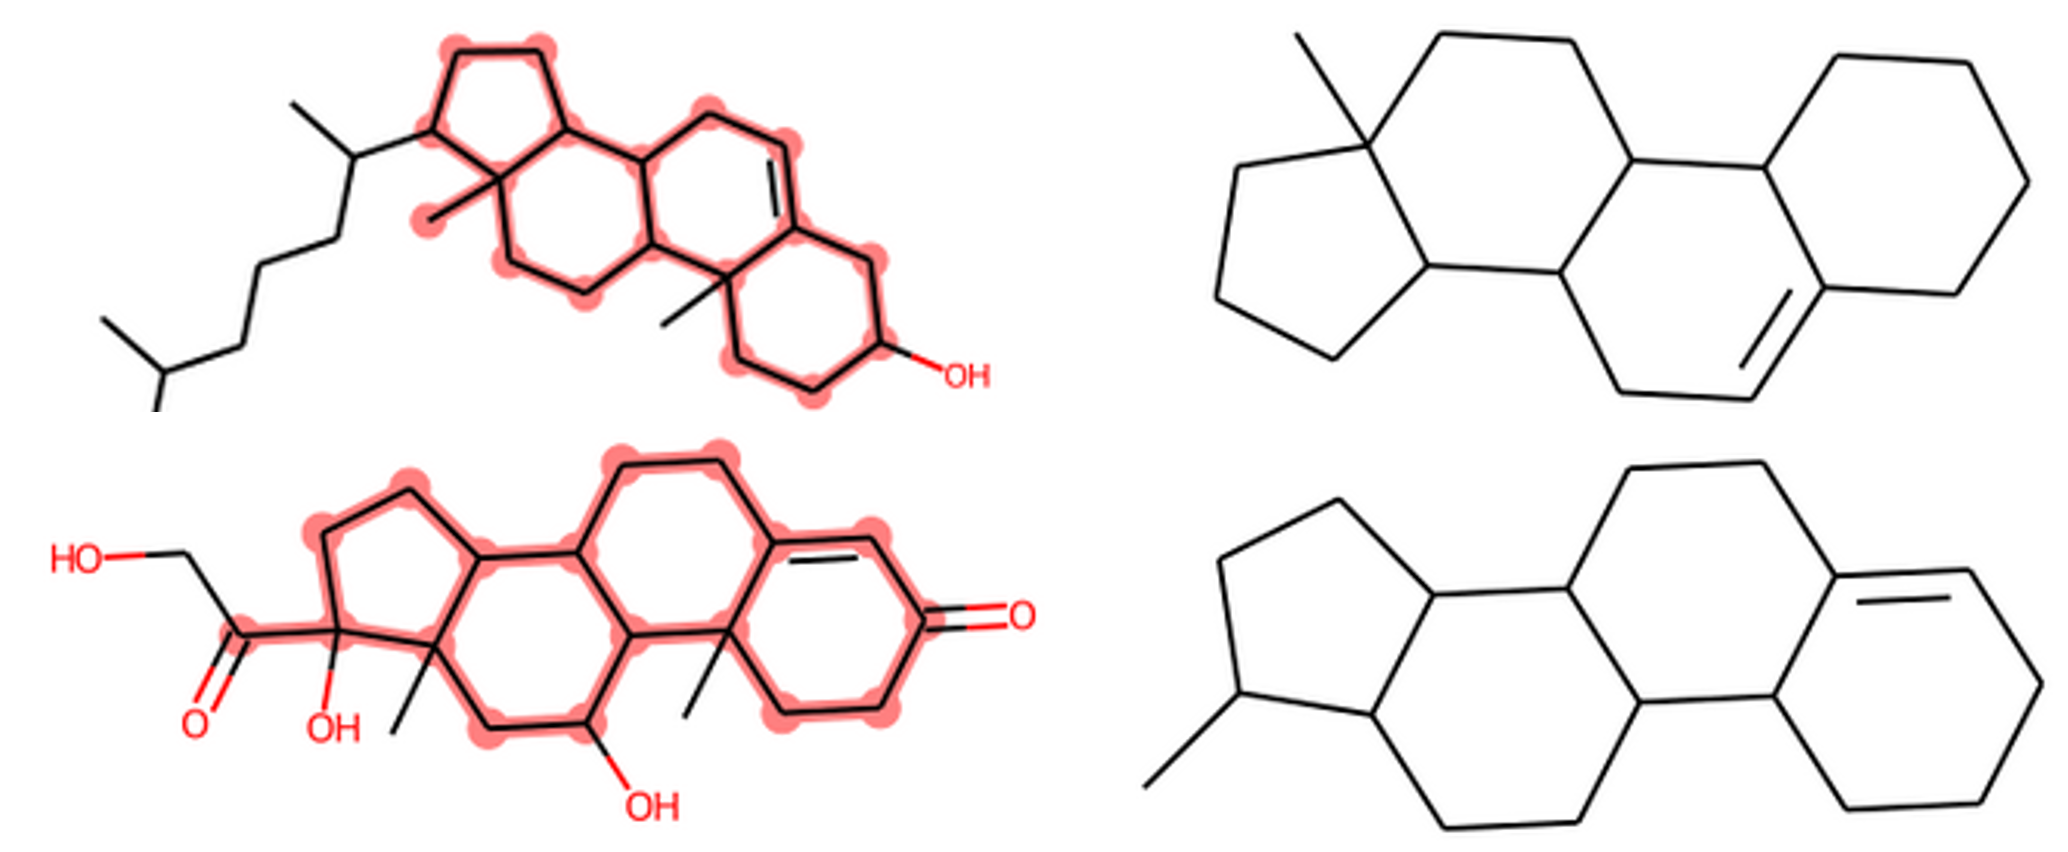
\includegraphics[scale=0.45]{sterols_wo_strictfusion}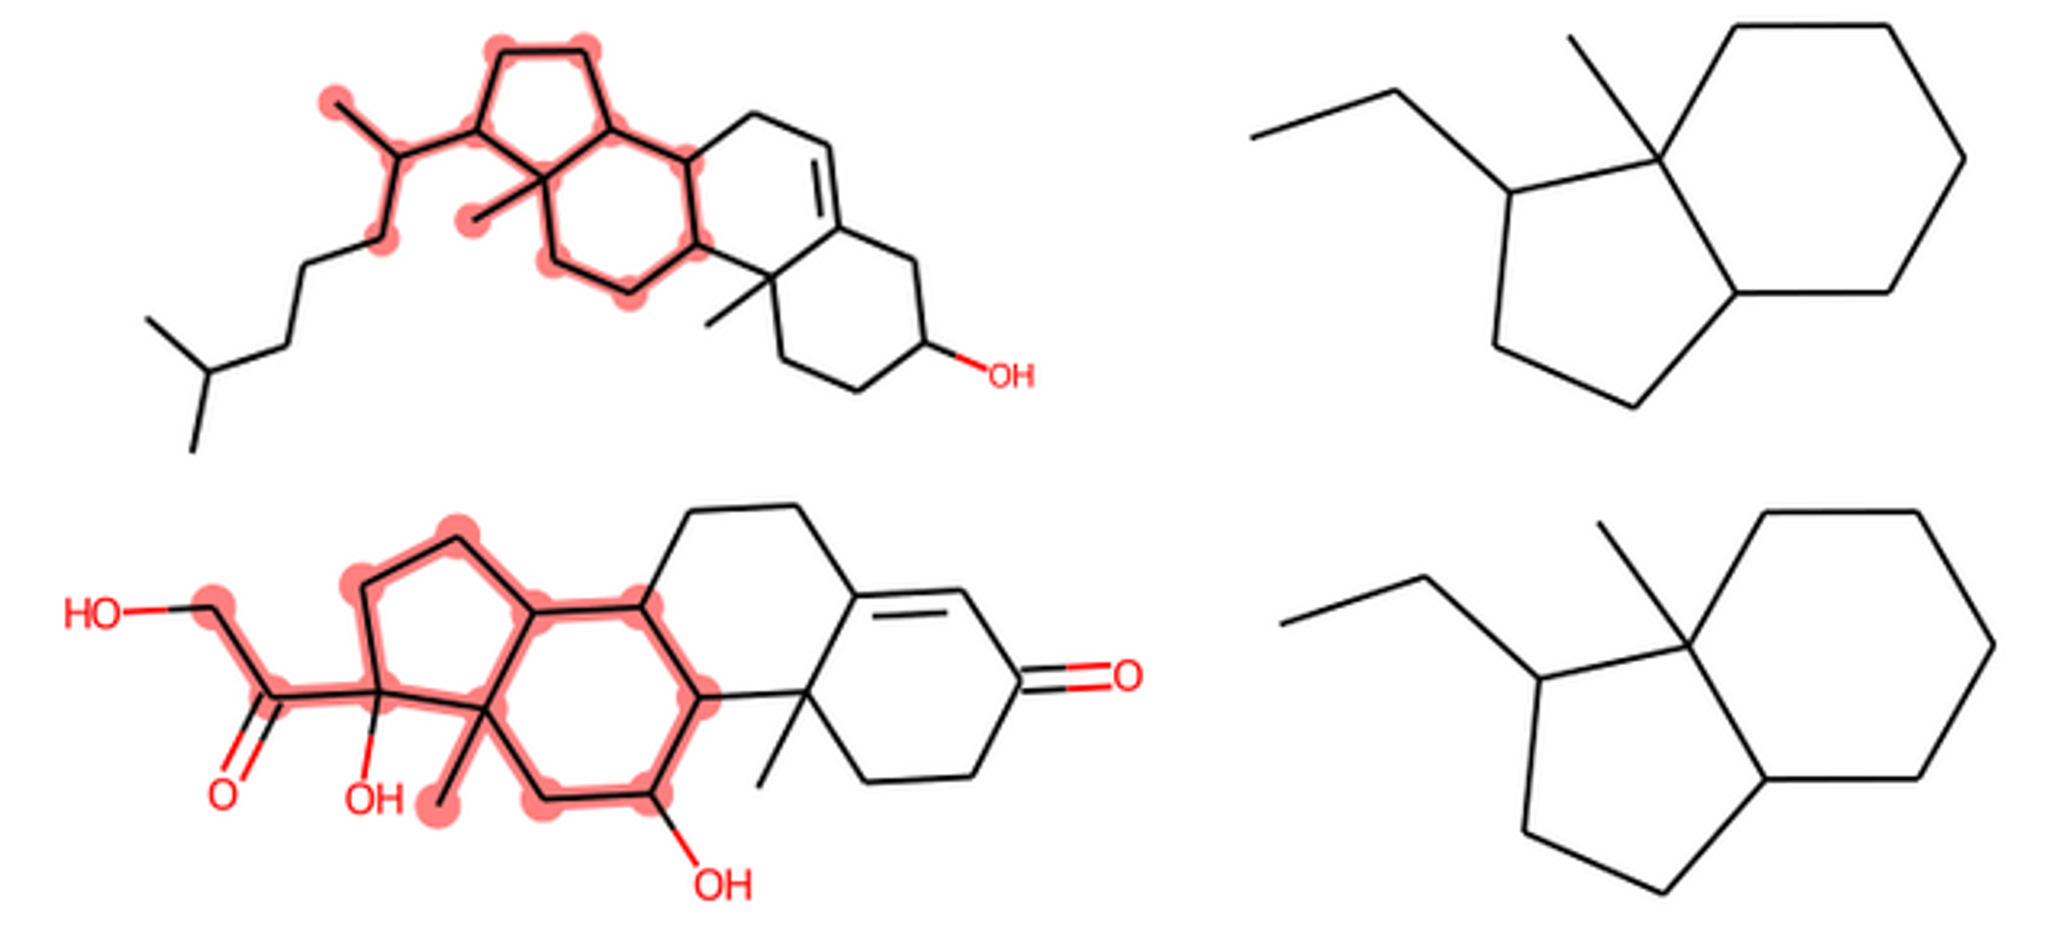
\includegraphics[scale=0.4]{sterols_w_strictfusion}

\caption{'Strict fusion' can affect the construction of the CC drastically, illustrated for cholesterol (top row) and cortisol (bottom row). First and second columns: CC of the two molecules without strict fusion; third and fourth column: common
core of the two molecules with strict fusion. In the images of the full molecule graph (first and third column), CCs are marked in red. In the example shown, none of the settings yield a valid CC for \trafo; the iterative approach explained in the main text would be necessary to obtain one. }
\label{fig:strictfusion}
\end{figure}




\begin{figure}
	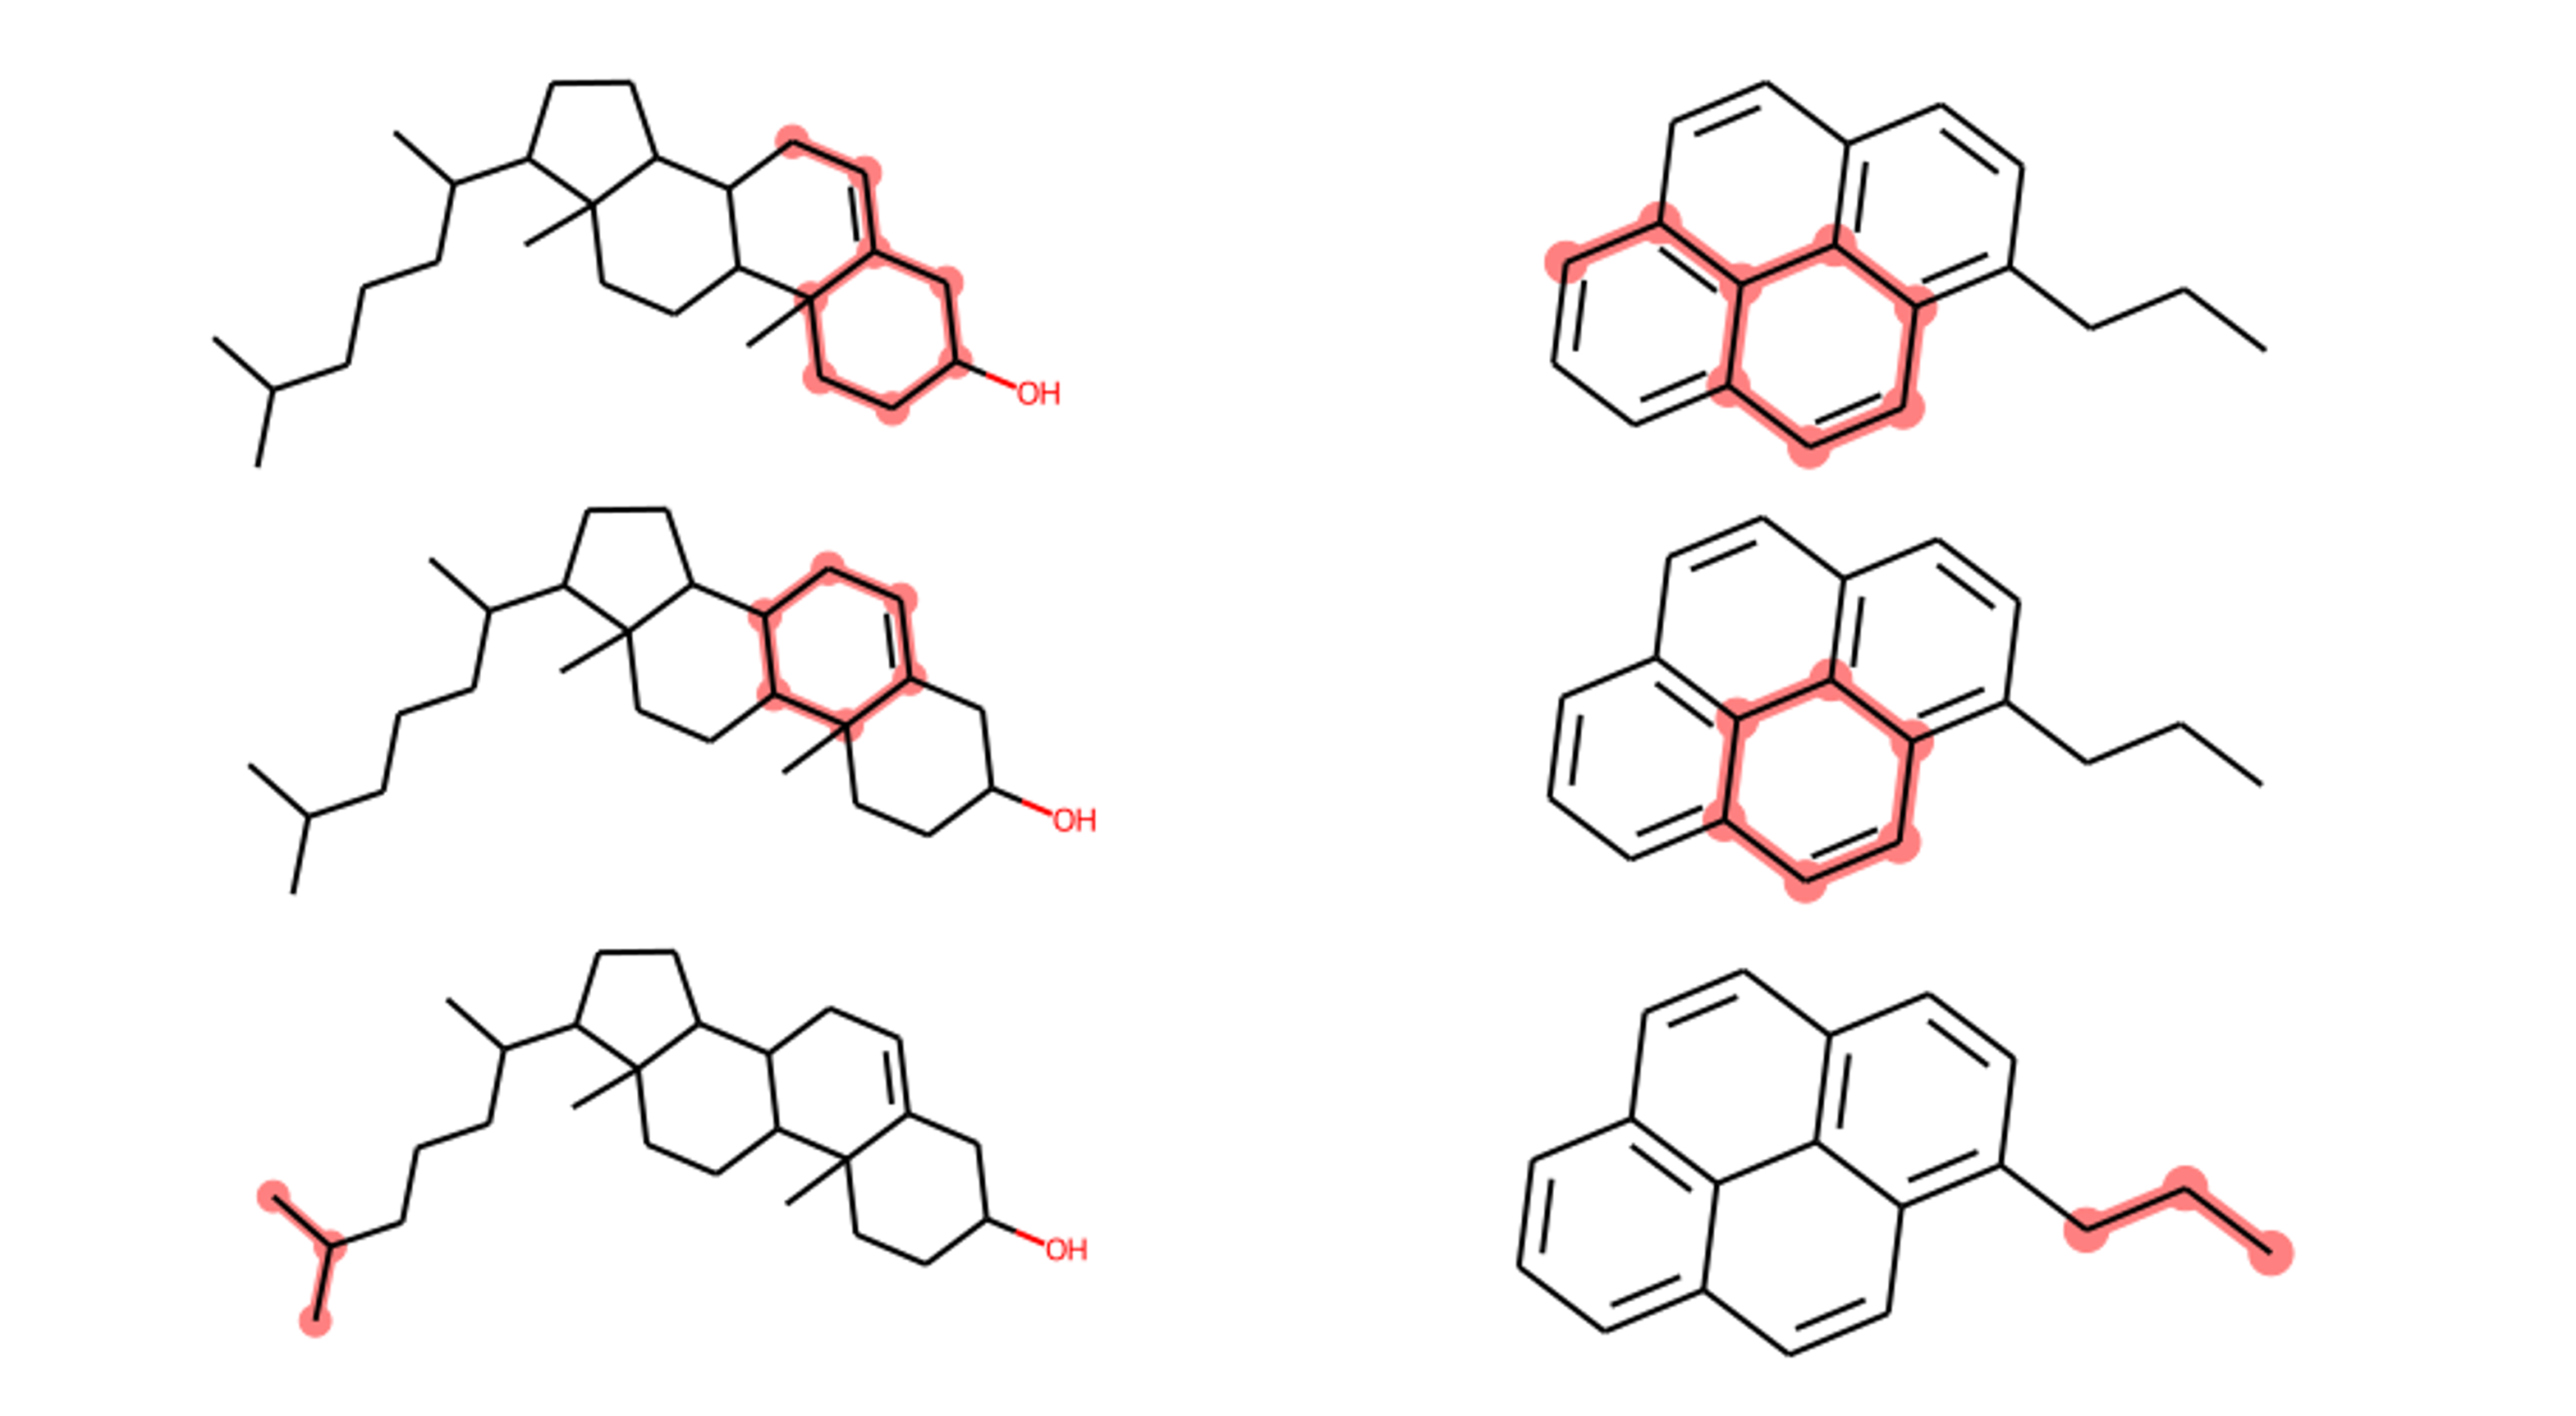
\includegraphics[scale=0.6]{cholesterol_pryenepropanoic_acid.png}
	
	\caption{CCs of cholesterol (left) and 1-propylpyrene (right); top row: CompleteRingsOnly = False; middle row: CompleteRingsOnly = True; bottom row: iterative approach to obtain a valid {\trafo} CC}
	\label{fig:pyrene}
\end{figure}


Of course, in the worst scenario, i.e., if both (non-identical) molecules only consist of ring-participating atoms, no valid CC for \trafo may exist. Similarly, the size of the valid CC may be tiny compared to that of the physical end states, which may make the CC approach as implemented in \trafo very inefficient.  In general, if at least one of the molecules solely consists of a polycyclic compound without any functional groups etc., and the other one does not have the same compound, no valid CC can exist. 
A --- maybe rather contrived --- example of such a pair of molecules and the construction of a valid CC via the iterative approach is given in fig.~\ref{fig:pyrene}. One sees that even the activation of the ring-related parameters of Rdkit is not sufficient to yield a valid CC, whereas the iterative approach gives the desired result. However, the resulting valid CC (which has the maximally possible size) is small compared to the original size of the molecules, despite the apparent similarity between both structures.



\section{Graph algorithms}

Using NetworkX and Rdkit, the molecules and their CC are
represented as graphs (in which nodes indicate atoms and edges bonds
between them). The selection of the optimal mutation route can be
understood as a graph traversal problem, in which the constraints mentioned
above are either implemented via the weights of the edges or by sorting.
Hence, the main task was to find suitable algorithms and graph initializations
to ensure an optimal processing of the mutation path.

Depth First Search (DFS) follows each chain of the graph as long as
possible, i.e., until a leaf node is reached. In contrast, Breadth
First Search (BFS) explores all chains simultaneously \cite{Even.2012}.
Problems and differences of both algorithms are illustrated using
several examples below. As will be discussed in more detail, the main problem of DFS is that it produces undesired outcomes. Often, heavy atoms near or next to the CC atoms are processed during the first steps of the graph algorithm, which may lead to an early opening of rings. Processing is completed only at a (much) later stage. Phrased differently, atoms are turned into dummy atoms in a highly 'asymmetric' manner.   

In each of the algorithms implemented, the root of the graph traversal is the node which connects the dummy region and the CC, i.e., the junction atom 'X'.
The shortest paths to all nodes of the dummy region are determined.

\begin{figure}

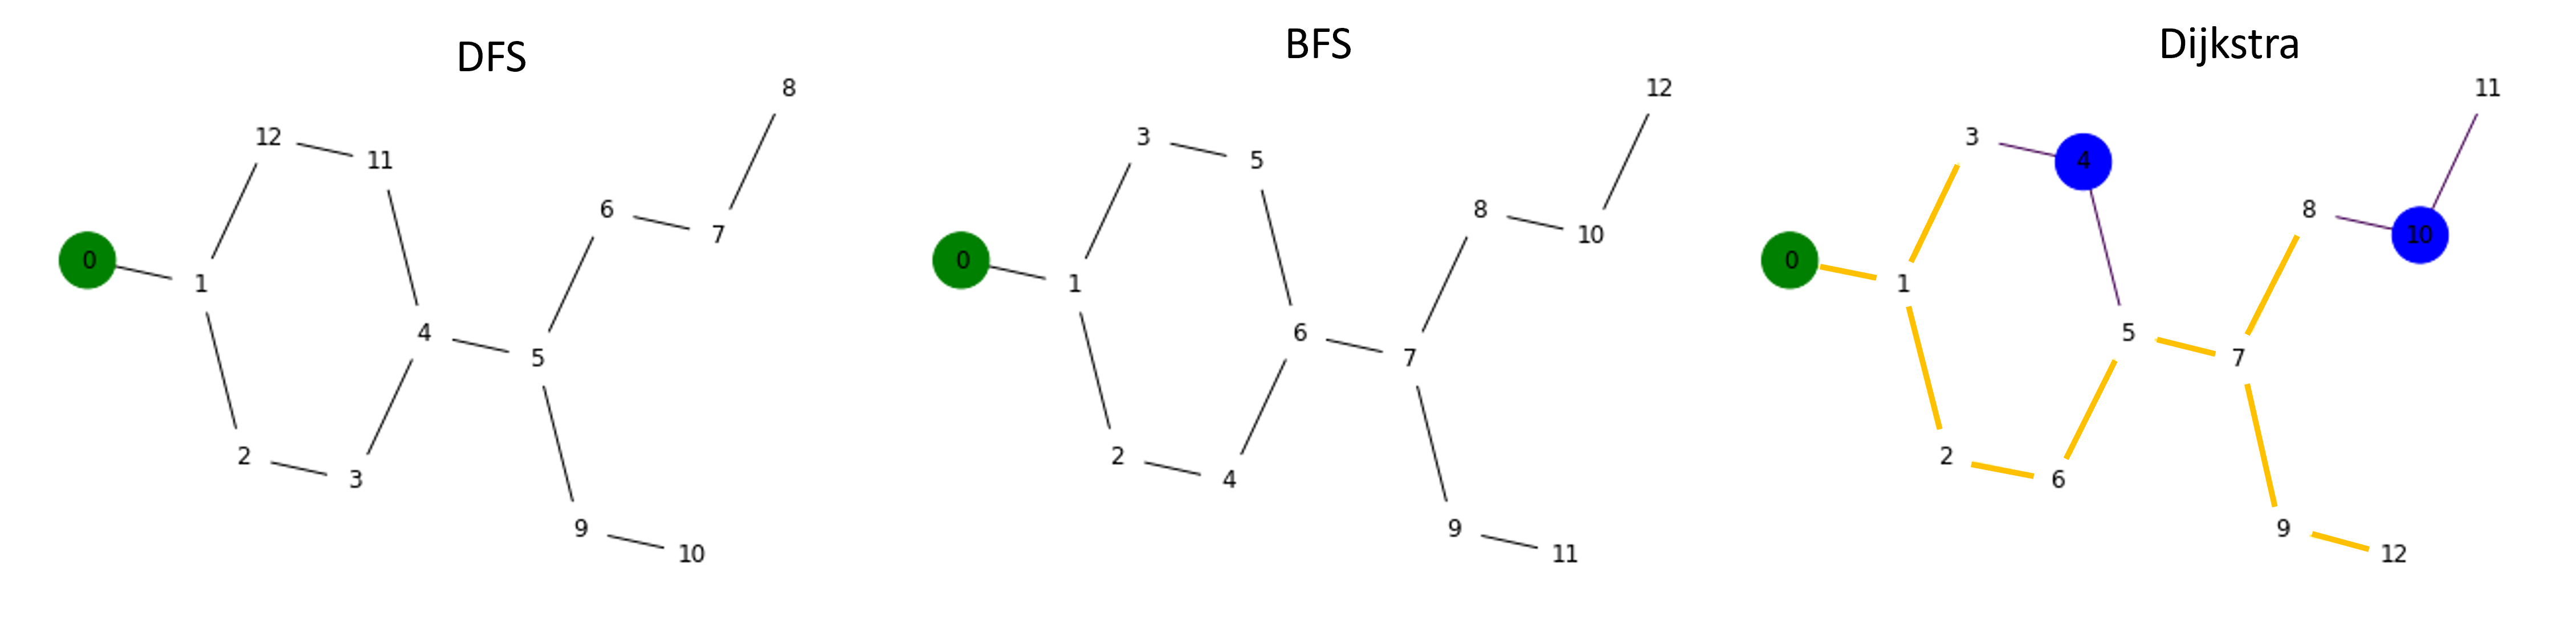
\includegraphics[scale=0.455]{dfs_bfs_dijkstra_comp1_v3.png}\caption{Comparison of different graph traversal algorithms. Green nodes represent the root atom; left: depth first
search (DFS); middle: breadth first search (BFS); right: Dijkstra algorithm. In the Dijkstra algorithm, blue atoms have increased weights;  the
edges connecting blue colored nodes have increased weights leading
to a mutation route differing from BFS; in the \trafo workflow, the final processing of the
nodes happens in reversed order; i.e., the atom first visited is removed last}

\end{figure}

The longest of these shortest path identifies the node which has the greatest
distance from the root (i.e., the atom with the greatest distance from
the CC). Therefore, the last element of the list returned by the search algorithm indicates the atom which has to be removed first; hence, the list of mutations orders has to be reversed.

If weighted graphs are used, the Dijkstra algorithm can be applied.
It finds the shortest path between two nodes or between a root node
and all other nodes of the weighted graph (the weights indicate the
edge length from one node to the other one). For unweighted graphs
(or, equivalently, graphs with uniform weights), the Dijkstra algorithm
reduces to BFS. Fig. 4.3 shows the different routes for modified weights.
In the test cases presented below, all graphs are initialized with uniform weights.

\section{New functionality added}

\subsection{Functions for creating mutation paths}

To use the newly implemented mutation algorithms, initially the graph object
is created with weights according to the atom type stored in a dictionary. The simulations shown
below use uniform weights; hence all atom types are treated equally; however, it is possible to modify these to
enforce a specific mutation route (e.g., accelerating or postponing
the exclusion of heteroatoms). 

The core functionality is given by the mutation processing functions.
Currently, three new functions are implemented, in addition to
the simple, existing DFS-approach.
These four main functions for computing mutation routes are:

\begin{enumerate}
\item \texttt{\_calculate\_order\_of\_LJ\_mutations:} this function performs the DFS algorithm, which has been used previously in {\trafo}. It may lead to  defective mutation routes (various examples are shown below and compared to the routes created by improved algorithms) and hence
should only be used for test purposes. The other three algorithms
are new, and all of them resolve most of the problems of the earlier
algorithm (especially isolated removal of ring atoms).


\item \texttt{\_calculate\_order\_of\_LJ\_mutations\_new:} the BFS/Dijkstra-algorithm is
applied once for creating a mutation route.

\item \texttt{\_calculate\_order\_of\_LJ\_mutations\_new\_iter:} the BFS/Dijkstra-algorithm is
applied iteratively, i.e., after each removal of an atom until all atoms of the dummy regions are processed.

\item \texttt{\_calculate\_order\_of\_LJ\_mutations\_new\_iter\_change:}
similarly to the last function, this approach works iteratively. In contrast to \texttt{\_calculate\_order\_of\_LJ\_mutations\_new\_iter:}, after each removal of an atom, the algorithm/routine for the next step is chosen depending on the current state, e.g., if the last processed atom belongs to a cycle or a chain.
\end{enumerate}

These functions
can be further modified by passing arguments which activate some helper
functions.These functions like \texttt{cycle\_checks} carry out tasks to ensure the
desired mutation route, e.g., count the number of cycles an atom participates
in. Further features of all algorithms are 'preferential removal';
i.e., if two atoms have the same priority (given by the current
weight) for the next mutation step, the weight of the atom which is
next to an already removed atom is updated so that this atom is excluded
next.

In the following, the most important of these functions are shortly described:


\begin{itemize}
\item \texttt{cycle\_checks(G)}: this function takes a NetworkX-graph object as input, checks which atoms participate
in how many cycles/rings and finally returns a dictionary with the atoms as
key and the number of rings the atom is participating in as value
and a dictionary with the degree (i.e., number of edges) of each atom
node. It is currently used in \texttt{\_calculate\_order\_of\_LJ\_mutations\_new}
(via the \texttt{change\_route\_cycles}-function).

\item \texttt{change\_route\_cycles\string(route, cycledict, degreedict, weightdict,G\string)}: this function is used in \texttt{\_calculate\_order\_of\_LJ\_mutations\_new}
and sorts nodes according to degree, cycle participation and information
about the nodes which have been removed immediately before. The preliminary mutation
path is sorted using a cycle and degree dictionary. If nodes have the same
weight (i.e., distance from root), the node participating in more cycles
is removed later. If nodes have the same weight (i.e., distance from root)
and same cycle participation number, the node which has more neighbors
already processed is removed earlier

\item \texttt{cycle\_checks\_nx(G)}: This function modifies the weight of
the graph, nodes participating in many cycles get lower weight. It
is currently used in 
\texttt{\_calculate\_order\_of\_LJ\_mutations\_new\_iter} and \texttt{...\_new\_iter\_change.} It returns a nx-graph-object
with updated weights (according to cycle participation of the atom).

\item \texttt{order\_checks\_nx(G, removearray, G\_total)}: This function
performs the 'preferential removal', if a node is connected to the
node removed in the last step, its weight gets a small increase so
that the removal of this node is prioritized. It is currently used
in\texttt{ \_calculate\_order\_of\_LJ\_mutations\_new\_iter} and returns
a nx-graph-object with updated weights.
\end{itemize}

If the \texttt{cyclecheck}-argument of the new mutation algorithms is set to True,
updates are updated according to cycle participation (as the systematic
processing of ring structures is one of the central goals, this functionality
should always be enabled, except for comparison and test purposes).
If in the case of \texttt{\_calculate\_order\_of\_LJ\_mutations\_new
and \_calculate\_order\_of\_LJ\_mutations\_new\_iter} also ordercycles
or ordercheck, respectively, are set to True, weight updating according
to preferential removal decides that the node in which neighborhood
nodes have already been turned off is removed next if there is no
possibility to decide between two nodes --- i.e., the weight of both
would be the same.

In each algorithm, all nodes of the graph (i.e., atoms) are usually
initialized with the same weight (e.g., 5). Alternatively, the user
could also pass an individual dictionary with different weights for
each atom type.
For the graph algorithms, NetworkX is used. For example,
the BFS- / Dijkstra-algorithm starting from the node connecting common
core and dummy region is implemented via the NetworkX-function \texttt{single\_source\_dijkstra}
which determines the path length of all dummy nodes to the root.

The main difference between these algorithms is that in \texttt{\_calculate\_order\_of\_LJ\_mutations\_new\_iter}
and \texttt{...\_iter\_change} the graph traversal part performed
using the Dijkstra algorithm is applied after each exclusion step; i.e., $n!$ atoms are visited instead of $n$; even for relatively large molecules the additional computational cost is negligible, in particular in comparison
to the computational time needed for the search of the CC.
The advantage of the iterated version is that after each mutation step, weights can be
updated or even the search algorithm can be modified. 

This feature allows for different mutation strategies depending
on the current state. Such an approach is demonstrated in \texttt{\_calculate\_order\_of\_LJ\_mutations\_new\_iter\_change}.
In contrast to the other algorithms, the algorithm processes information
if the last removed node was part of a chain or a cycle. Depending
on the state, the chain, or cycle, is processed fully before the algorithm
moves on to other parts of the molecule. Fig. \ref{fig:iter_iter_change_comparison} demonstrates the difference between the two versions of the iterated algorithm.
Whereas in the non-iterated algorithm the found mutation route has to be reversed (since the atom node with the highest distance from the root is the first which has to be turned off), in the iterated versions at each iteration the node with the highest distance is added to an array which determines the final mutation route.

The computed mutation routes can be visualized directly via Rdkit. 
The route is represented by a color gradient used for the atoms involved
in the mutation process (\texttt{\_show\_common\_core\_gradient}). By default, the color spectrum ranges from red to green; the first atom to be removed is colored red, the last green.

Furthermore, an animated 3D-visualization of the mutation process
is implemented using py3Dmol (\texttt{animated\_visualization\_3d\_v2})\cite{key-4}. 



\subsection{Processing of hydrogen atoms}


As fig. \ref{fig:hydrogen_effect} indicates, the presence of hydrogens can influence the CC generation dramatically. In particular, the maximum common substructure for a molecule representation with hydrogens can encompass less heavy, i.e., non-hydrogen, atoms than the substructure for a representation with hydrogens removed (although, including the hydrogens, the total number of atoms is higher in the first case). Hence, it is crucial to determine the CC for molecule representations without hydrogens. 
Since hydrogen atoms are turned off in an extra step en bloc during the {\trafo} workflow, the mutation route algorithm should not take hydrogens into account, nor must the CC be generated for a molecule representation containing hydrogens.
Nonetheless, it is necessary that the molecule representations processed by \trafo contain all hydrogens in explicit form because the indices of these atoms in the underlying data structures are used in some steps, e.g., for scaling the van der Waals interactions of the hydrogen atoms to zero.
This problem was solved by removing and adding hydrogens appropriately.
In a first step, the {\trafo} function determining the CC (\texttt{\_find\_mcs} in mutate.py which is the Python file containing most {\trafo}-functions responsible for generating the CC and the mutation paths) had to be modified. 

To obtain the desired CC but retain the {\trafo} workflow, the following scheme was implemented:
A deep copy of both molecules is created. The hydrogens of these copies are removed; then their CC is computed. For both molecules, the indices of the atoms corresponding to the CC are determined. Finally, it is checked for each CC atom of both molecules whether hydrogen atoms are in its neighborhood. If such hydrogens are found, their indices are added to the lists of CC atoms. These lists of atoms, including hydrogens, are stored for both molecules and the function returns the maximum common substructure (determined for the molecules without hydrogens).
Thus, the procedure yields the necessary output for further processing in {\trafo}: The molecule representations and lists of CC atoms for both of the molecules include hydrogens, but the maximum common substructure giving rise to the CC is computed only for the heavy atoms.

Similarly, the functions for computing the mutation routes had to be adapted for input molecules containing hydrogens. By default, a helper function removes the hydrogens from the graph representation as well as the corresponding indices from the list with the atoms of the dummy regions before the mutation algorithms are applied. Afterward, the hydrogen atoms adjacent to CC heavy atoms are added to the CC.

A special problem occurs for molecule pairs with switching 'X'-atom; fig. \ref{fig:pyrrolidinindole} shows 2-/7-pyrrolidinindole as an example. The red highlighting shows a correct CC for both molecules; in each of them one should note the hydrogen atom, which is directly bonded to one of the CC-carbon atoms, but itself is not part of the CC. If the hydrogens were added, the CC would not be valid anymore: It is necessary that a further dummy region emerges which consists solely of one hydrogen atom because otherwise the CCs would have a different number of atoms and would not be isomorphic anymore. If, however, the CC is generated without hydrogens, the information which of the hydrogens turns into a dummy region is lost and the construction of a valid CC cannot be assured.
It has to be stressed again that the presence of these hydrogen dummy regions does not affect the mutation steps, but is nonetheless crucial for the internal {\trafo} workflow. 

However, there is a straightforward way to circumvent this problem: From the substructure matches, the mapping between the CC atoms of each molecule can be read off. It is counted for each heavy CC atom how many hydrogens are connected to it. Finally, the minimum number of hydrogens is added to the CC. (In the case of 2-/7-pyrrolidinindole, this means that for each CC atom one hydrogen is added, except for the 2- and 7- position because for these positions in one molecule no hydrogen is connected).
In this context, also the difficulty that there are possibly many substructure matches has to be mentioned.

It is even possible that substructure matches differ solely regarding hydrogens. For this case, a parameter was added to the function which searches for the maximum common substructure. If \texttt{iterate\_over\_matches} is set to true, one of the substructure matches with most hydrogens, i.e., the biggest possible substructure, is selected. Fig. \ref{fig:neopentan} shows two CCs, only differing in the number of hydrogens.


\begin{figure}
	
	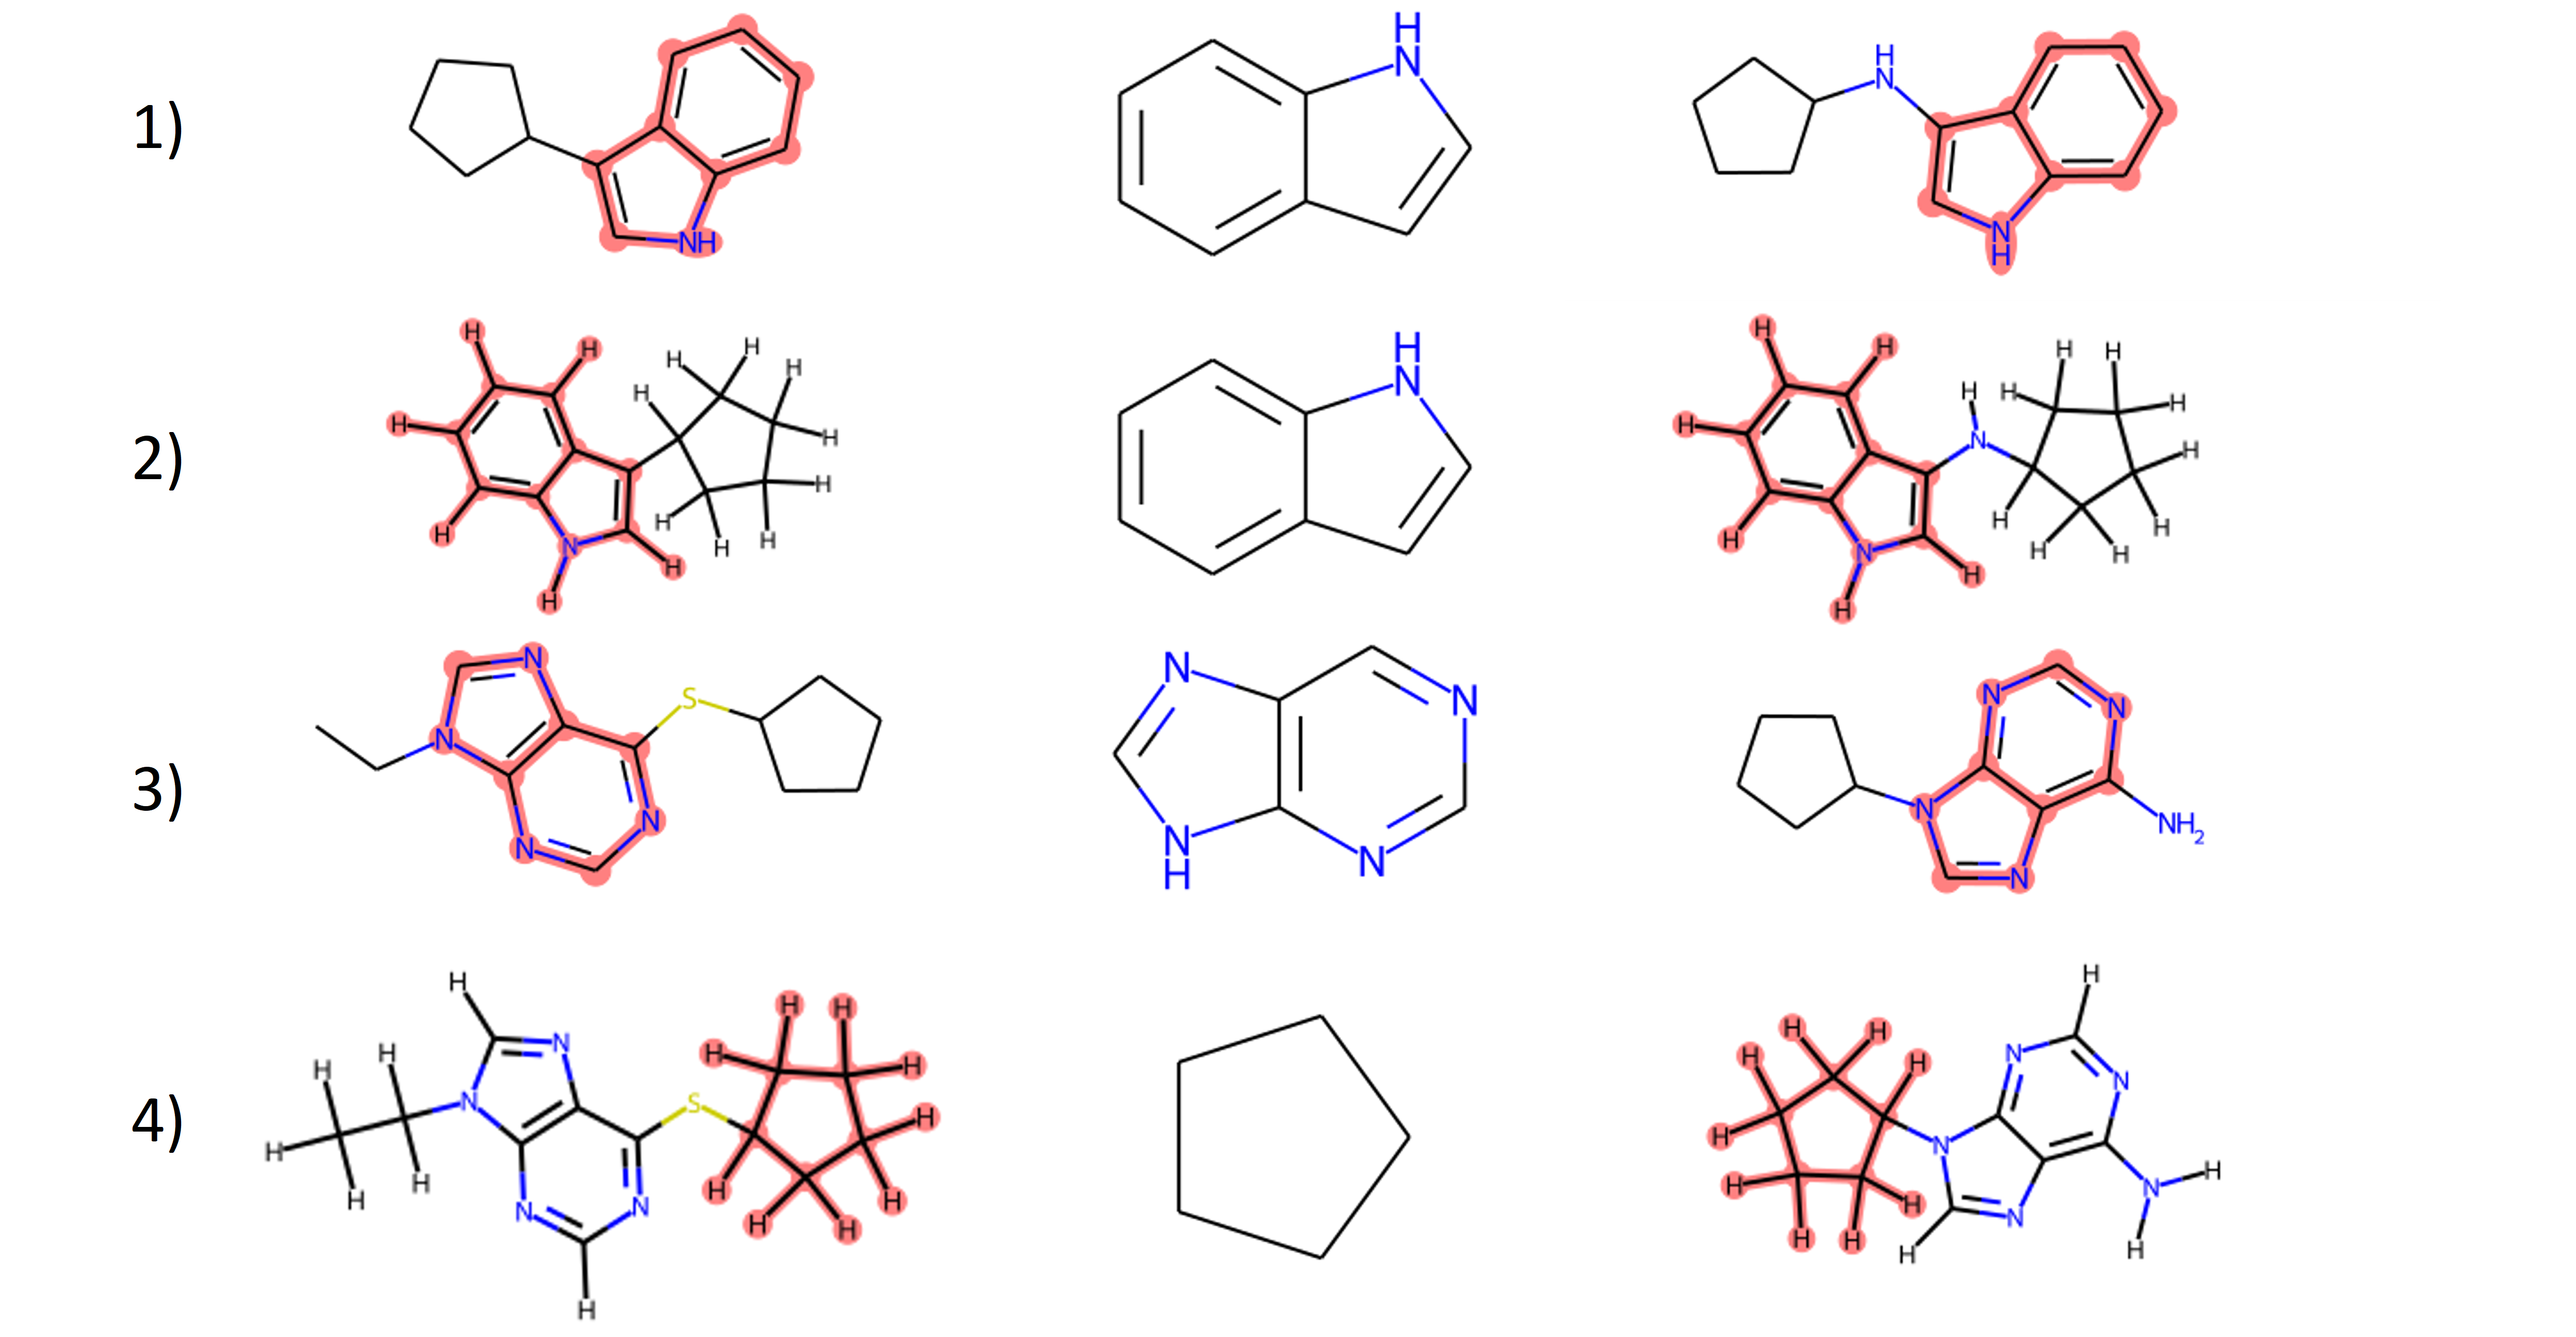
\includegraphics[scale=0.13]{hydrogens_plus_minus_v2.png}
	\caption{These examples demonstrate that the addition of hydrogens can influence the construction of the CC; left: molecule 1; middle: CC; right: molecule 2; in the representations of the full molecule, the CCs are marked in red; row 1)-2) and row 3)-4) show the same molecules, in the respective upper row without,
		in the lower with hydrogens; the CC of the molecule in row 3) and 4)  changes when hydrogens are added to the Rdkit-molecule
		representation}
		\label{fig:hydrogen_effect}
\end{figure}



\begin{figure}
	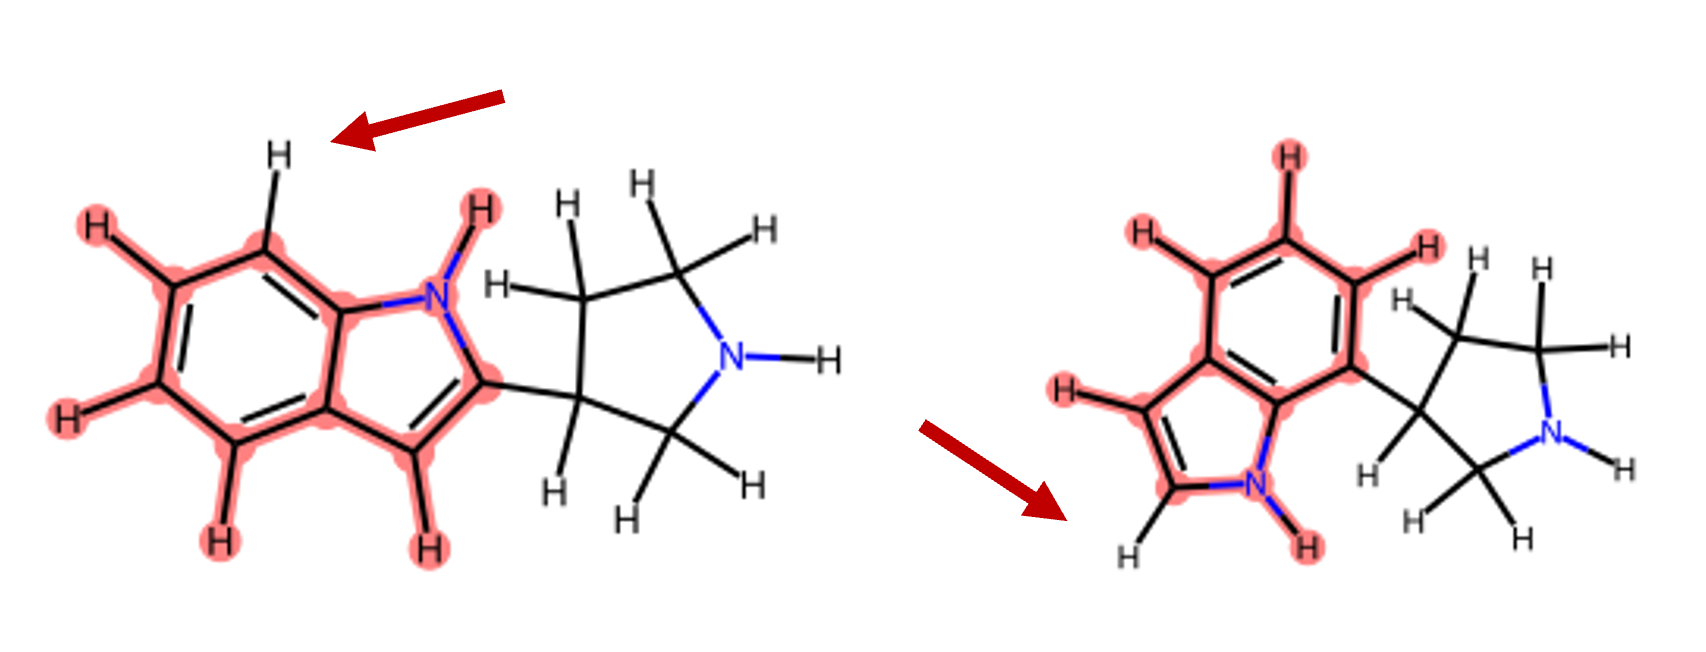
\includegraphics[scale=1.0]{pyrrolidinindole_v2}
	
	\caption{
		left: 2-pyrrolidinindole; right: 7-pyrrolidinindole; 
		one of the hydrogens --- exactly the hydrogen atom which is placed at the position of the junction 'X'-atom at the other end state --- is not part of the CC (otherwise, the CC would be invalid)}
	\label{fig:pyrrolidinindole}
\end{figure}


\begin{figure}
	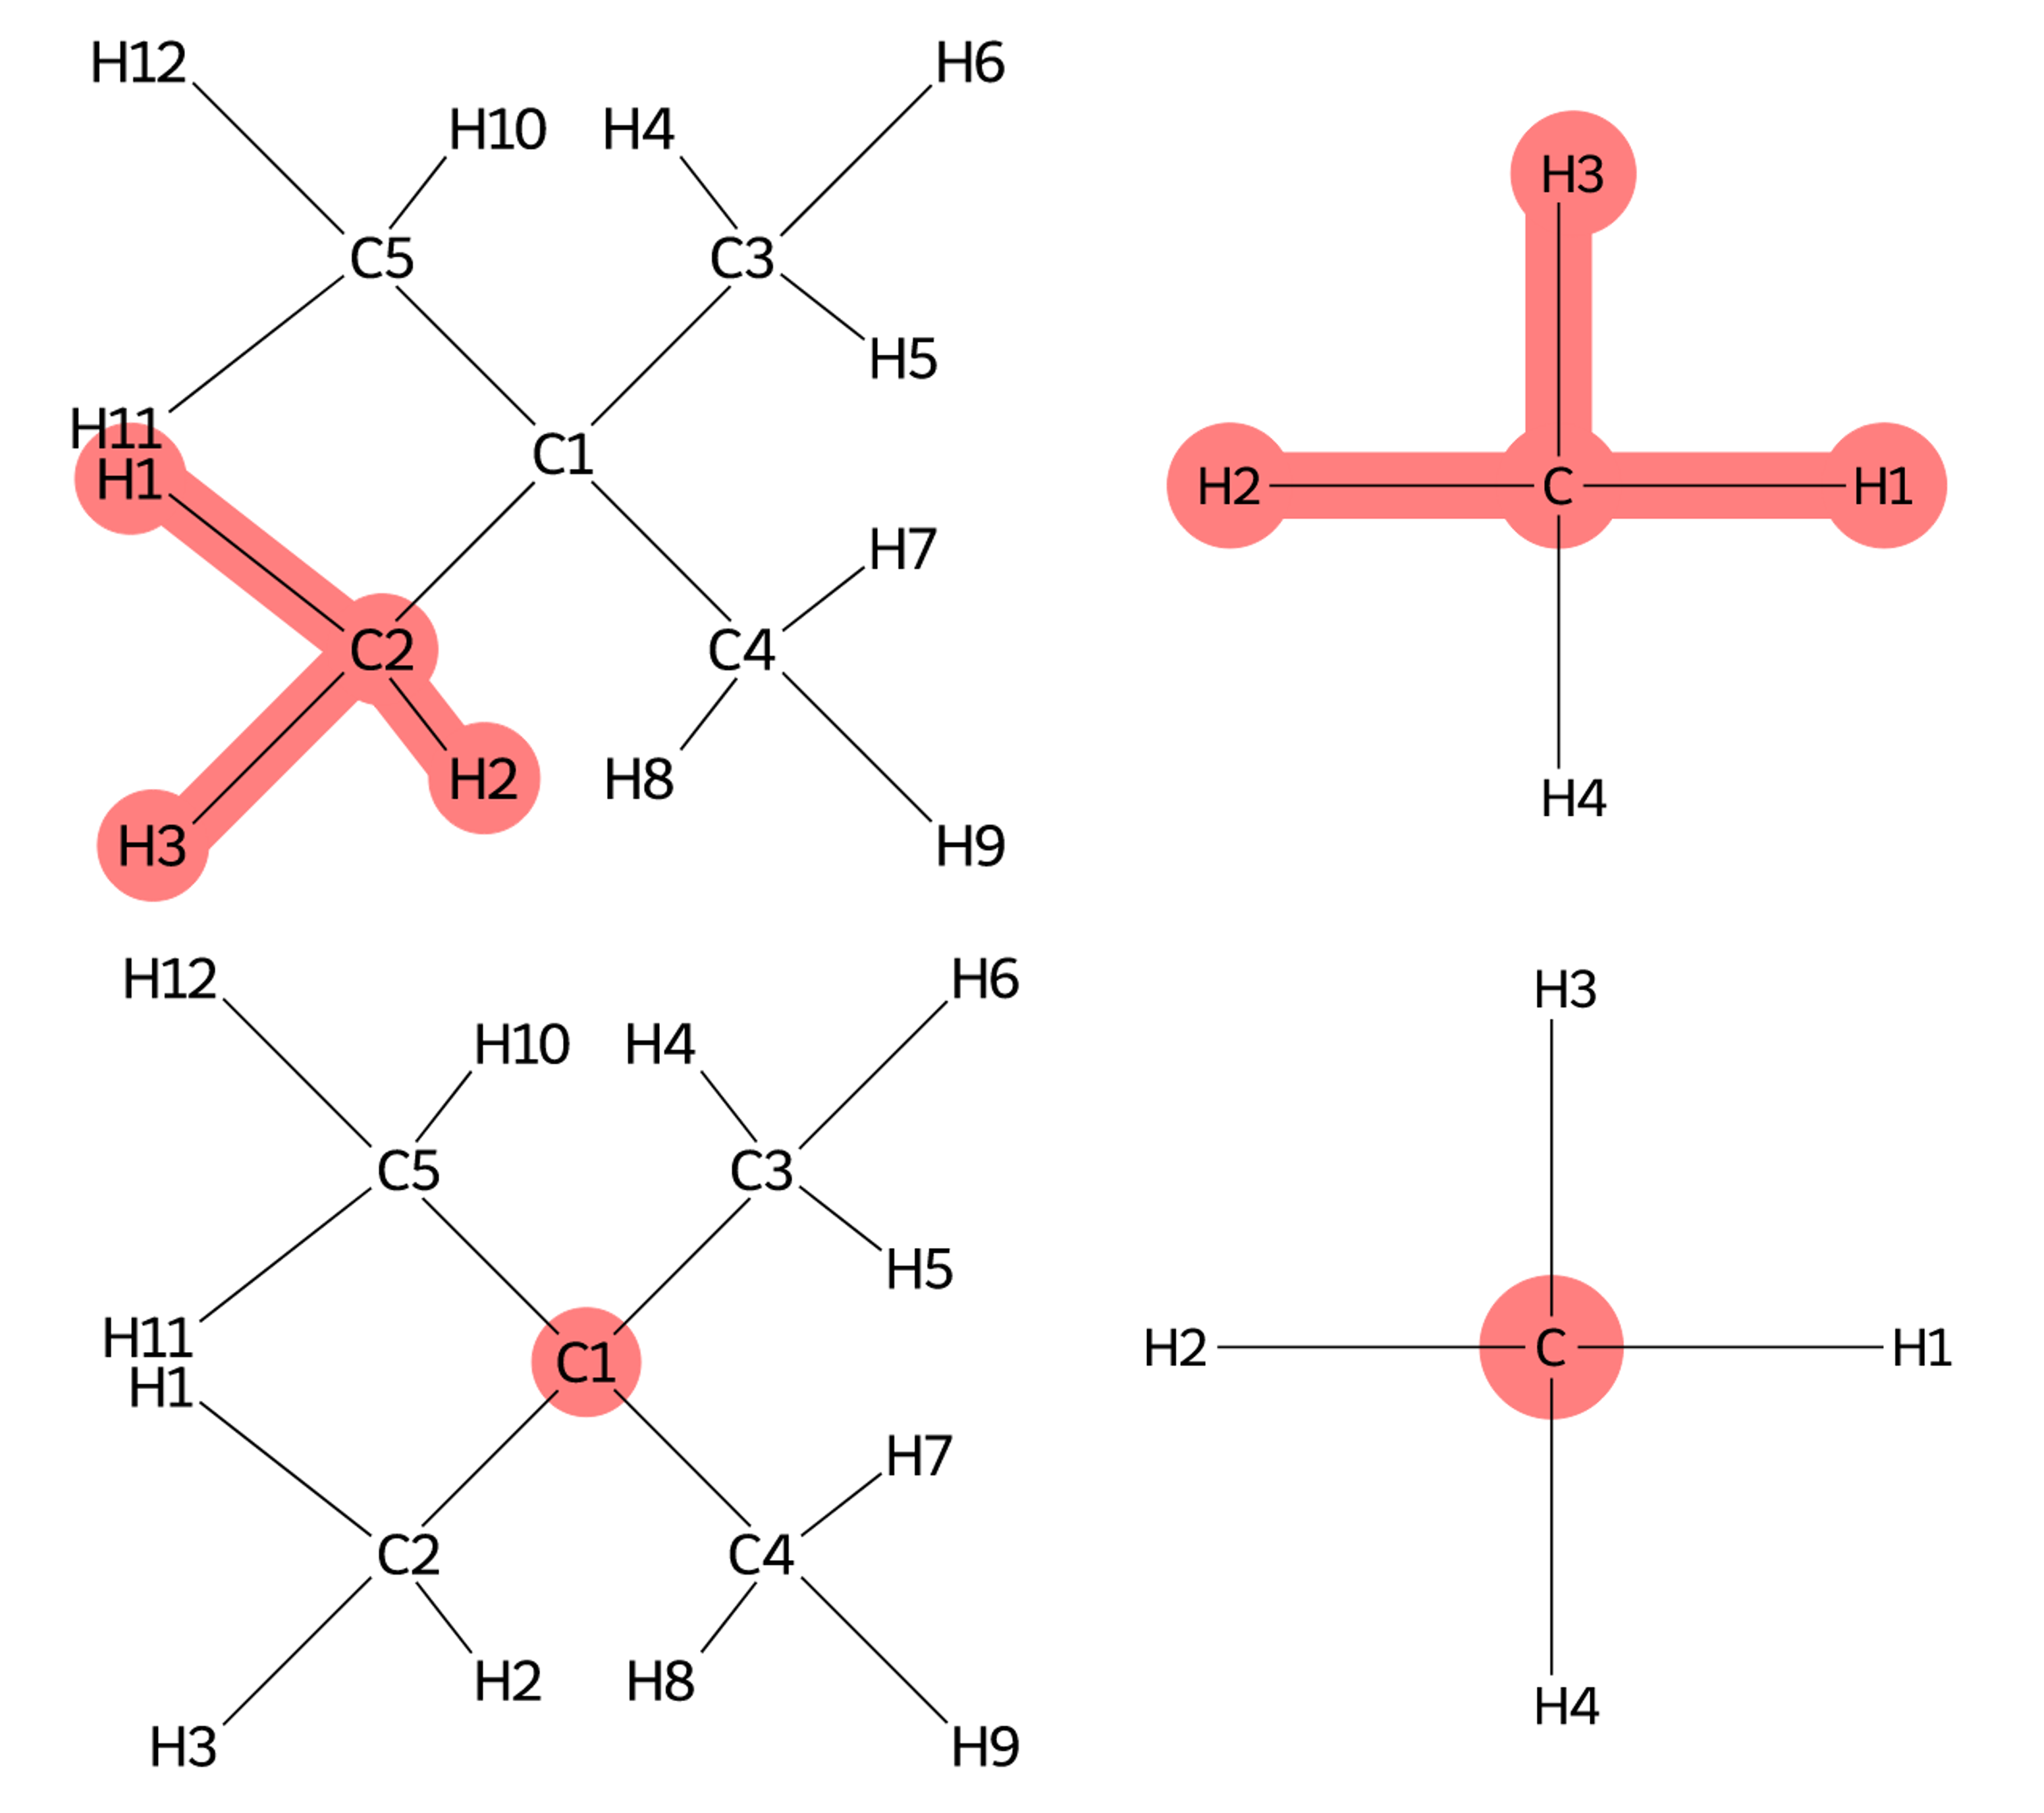
\includegraphics[scale=0.55]{neopentan_new}
	
	\caption{neopentane/methane CCs; upper row: CCs maximizing the number of atoms including hydrogens; lower row: CCs without considering hydrogens }
		\label{fig:neopentan}
\end{figure}



\subsection{Examples for processing molecules}

\begin{figure}
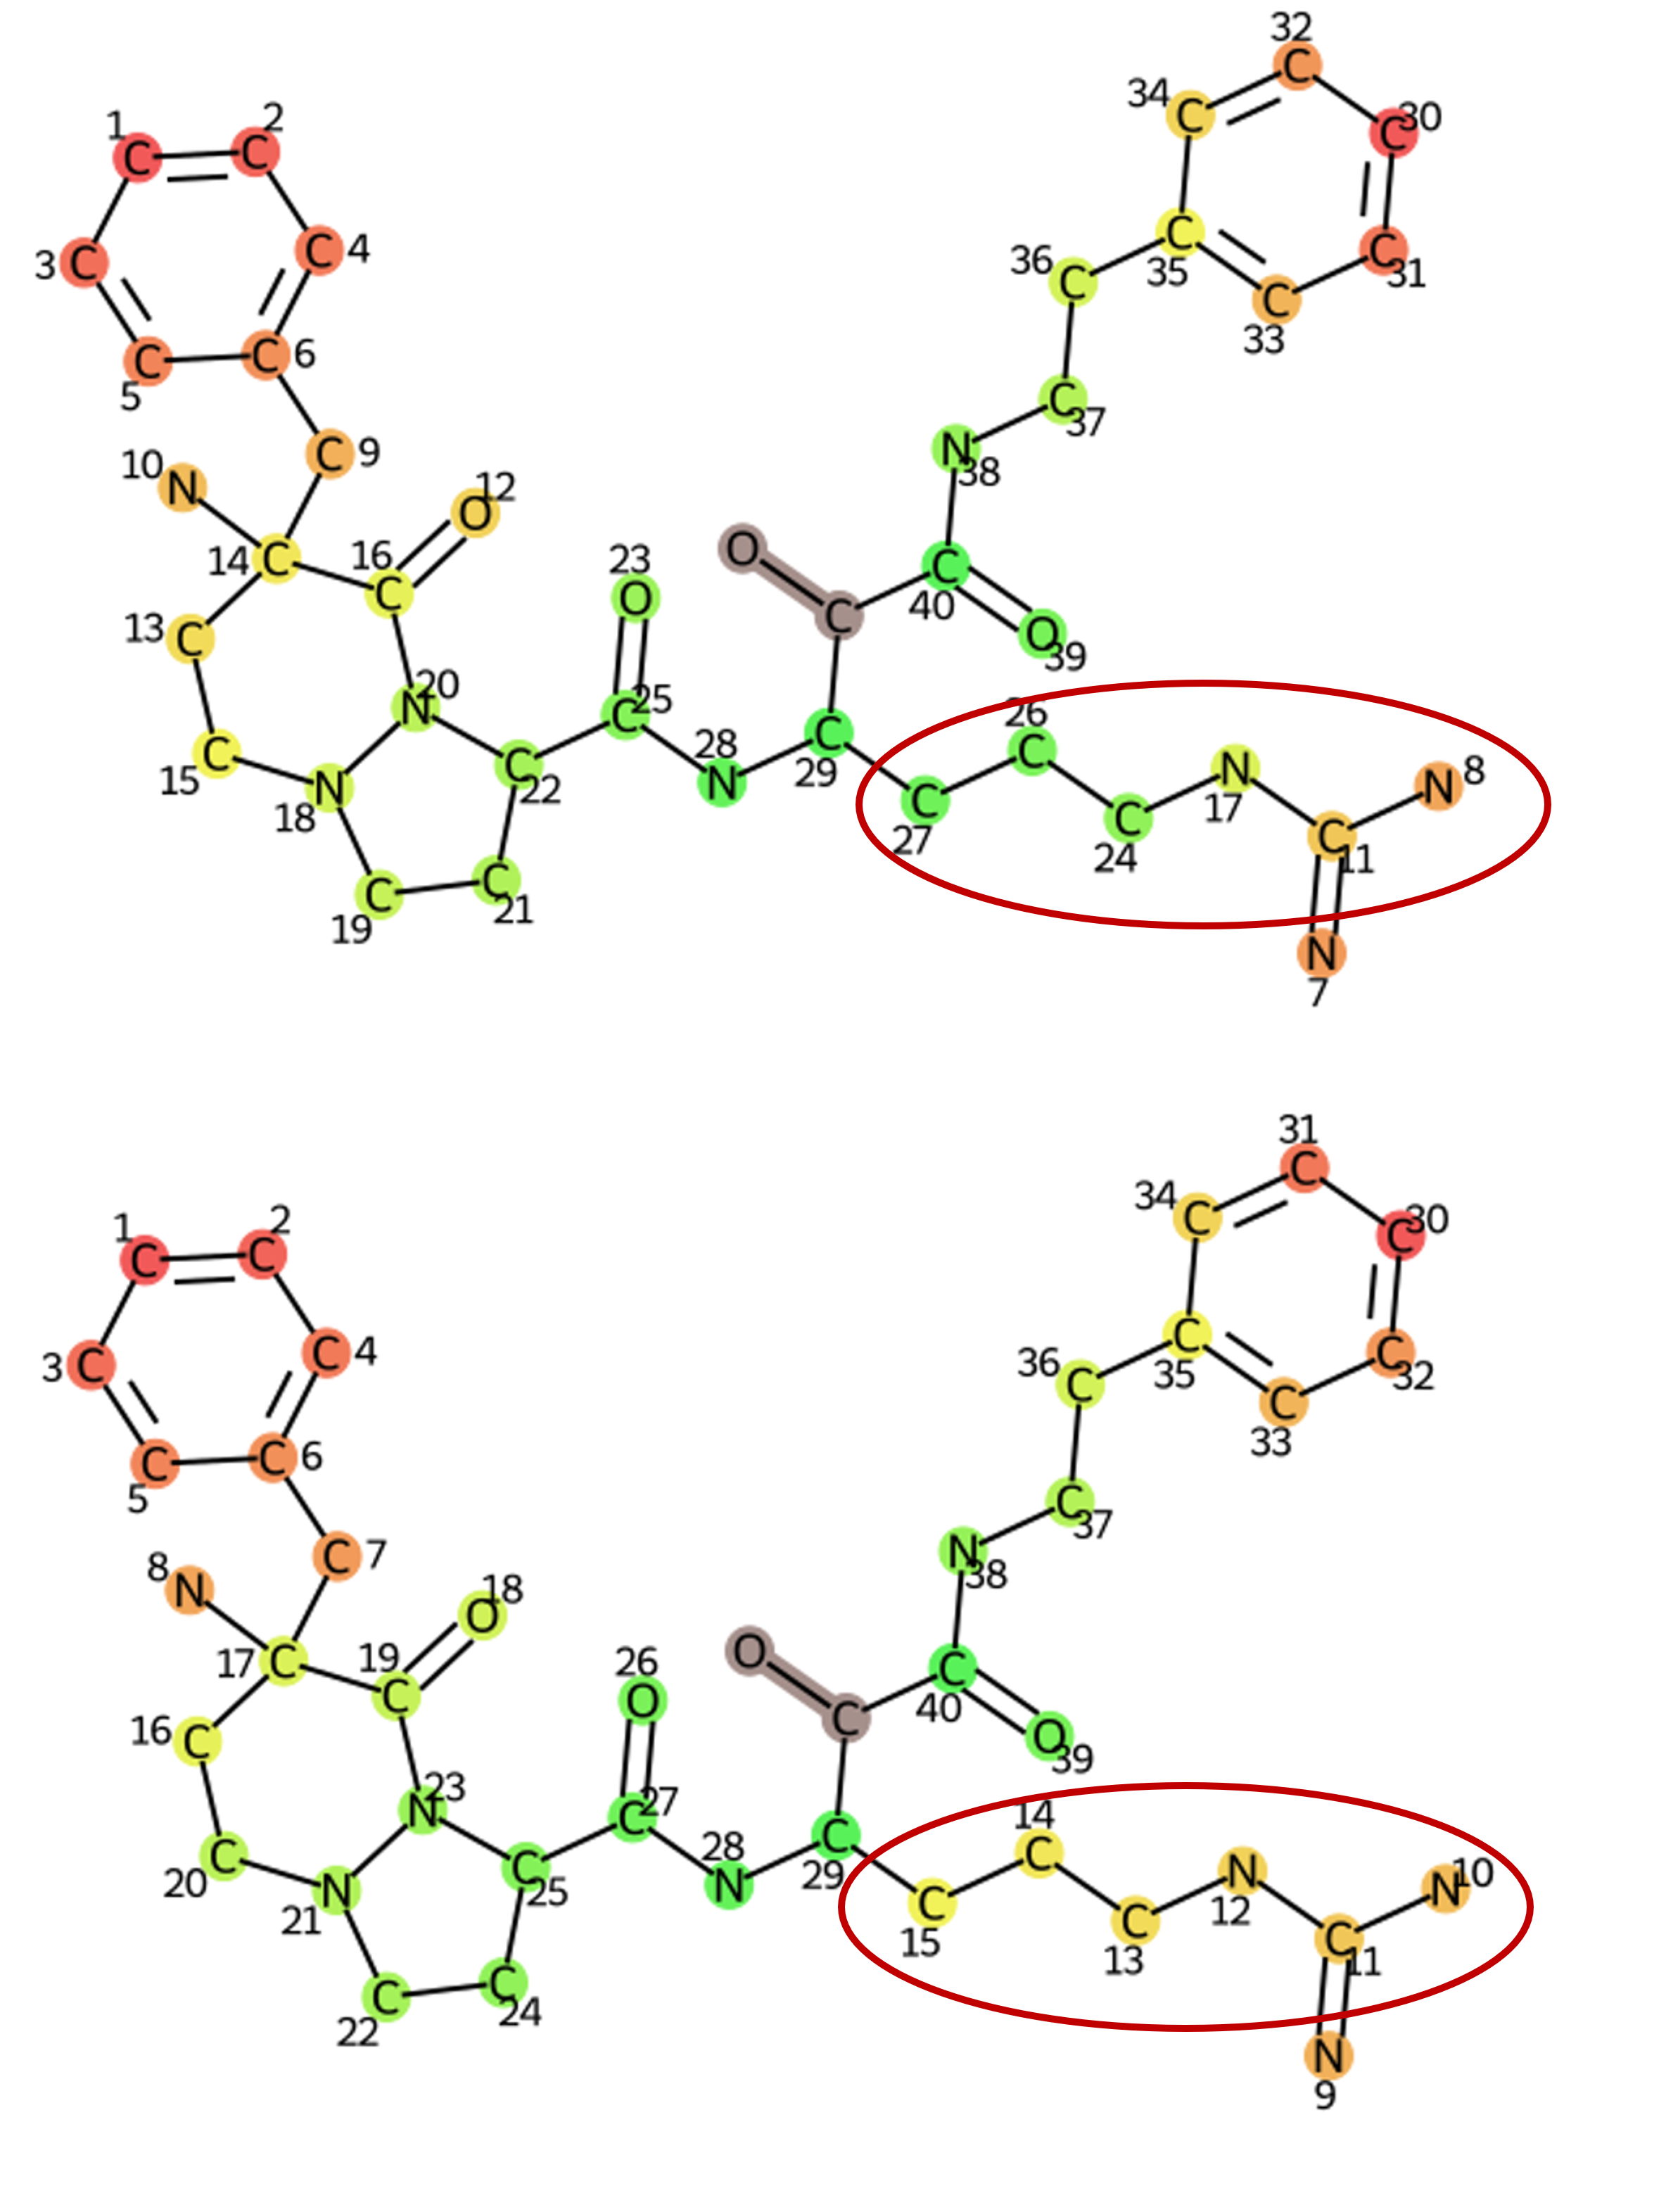
\includegraphics[scale=0.25]{iter_iter_change_1a5g_1_two_rows}

\caption{Example of the differences between the \texttt{iter-} and \texttt{iter\_change}-algorithms;
Top: \texttt{iter}; Bottom: \texttt{iter-change}; \texttt{iter-change }processes all atoms within
a chain or a ring at once (if possible) before switching to other
parts of the molecule}
\label{fig:iter_iter_change_comparison}
\end{figure}

As outlined above, in the current version of {\trafo}, one suboptimal route finding algorithm using DFS and several new versions based on BFS are implemented.
For single rings, BFS (or, in the case of different weights for various atom types, the Dijkstra algorithm) automatically processes the atoms in the most symmetric way starting at the atom with the highest distance from the root), whereas DFS gives rise to a long chain. Fig.~\ref{fig:comparison_dfs_bfs} illustrates this difference.
In more complex molecules, the systematic exploration of chains in
depth first search inevitably leads to big local gaps in processing
of the molecules. Fig. \ref{fig:simple_ring_exampledfs2} shows this problem for a benzene ring which
is directly attached to the CC. As DFS goes along one path
until the end; i.e., until a leaf node is reached, four atoms of the
ring are visited first, whereas the remaining two are explored
last. Therefore, these two atoms are turned off first, but then the
algorithm continues at a wholly different location and the remaining
ring atoms persist in the system until the end of the mutation process.
By contrast, BFS automatically produces the desired result for this system. 


\begin{figure}
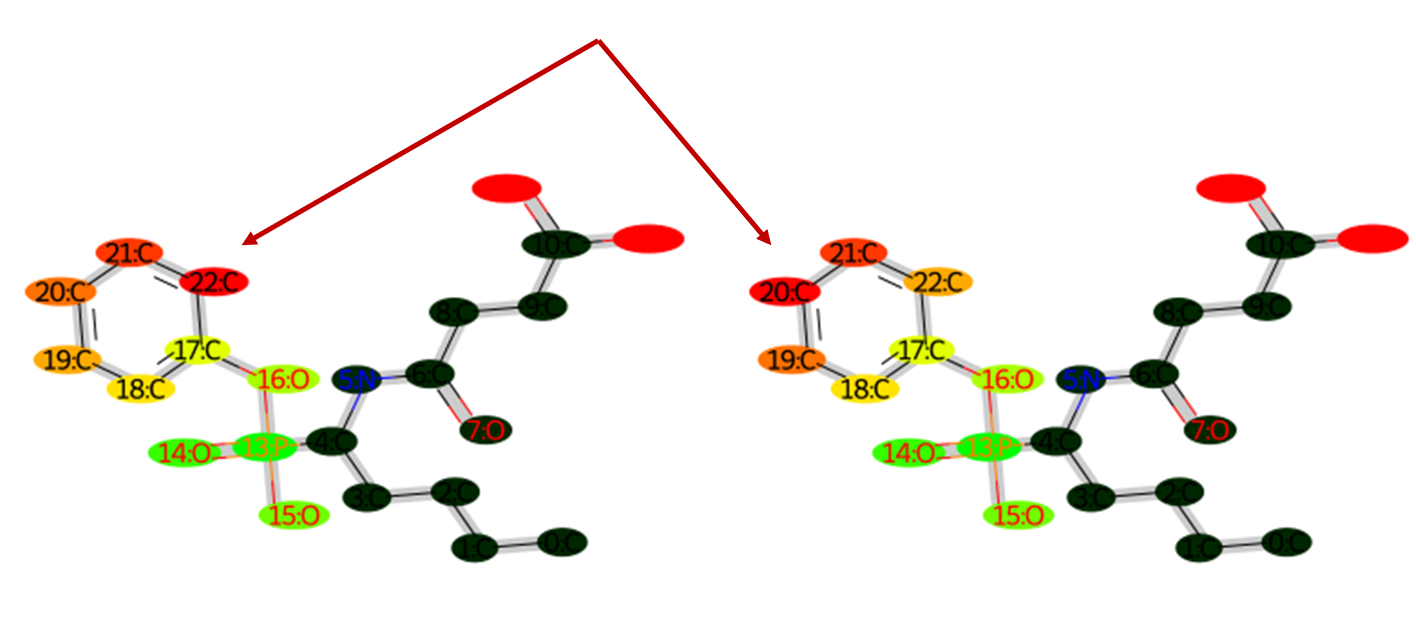
\includegraphics[scale=1.4]{simple_ring_exampledfs.png}

\caption{comparison of typical DFS- and BFS-mutation route for a single ring structure; left: DFS-algorithm; right: BFS-algorithm; in all depictions of mutation routes the CC is shown in dark, the color gradient starts at red indicating the atom first to be removed and ends at green; DFS
starts at the ring atom adjacent to the carbon atom bonded to the oxygen and thus ring breakage gives rise to one long
chain which is processed subsequently, whereas BFS starts at the ring position most distant from this carbon and the two emerging chains are processed in a symmetric fashion
}
\label{fig:comparison_dfs_bfs}
\end{figure}



Similarly, in fig.~\ref{fig:simple_ring_exampledfs3} one atom of the ring (marked by the red circle), adjacent to the X-junction, is omitted in the first exploration using DFS and only visited at last. Hence, it is first processed, whereas the other atoms of the ring are removed much later.

More complex ring structures exacerbate the problems. Fig. \ref{fig:simple_ring_exampledfs4} shows that also the processing of the substituents is affected.

Multiple rings pose special difficulties for the mutation algorithms because
the processing of one of the rings can easily lead to gaps in the adjacent
ones. Figs. \ref{fig:2ring_example} and  \ref{fig:2ring_example2} illustrate that severe problems may occur when using DFS.
As in the case of one ring, the exploration route implies that one
of the rings is opened in such a way that it gives rise to a lengthy chain.
Furthermore, an atom may belong to two or more rings is visited early, whereas other atoms of the ring are explored much later, so that both ring structures are opened
and teared apart (fig. \ref{fig:2ring_example}). Likewise, one half of each of the
rings is turned off many steps before the processing of the remaining ring atoms is done (fig. \ref{fig:2ring_example2}). 

\begin{figure}
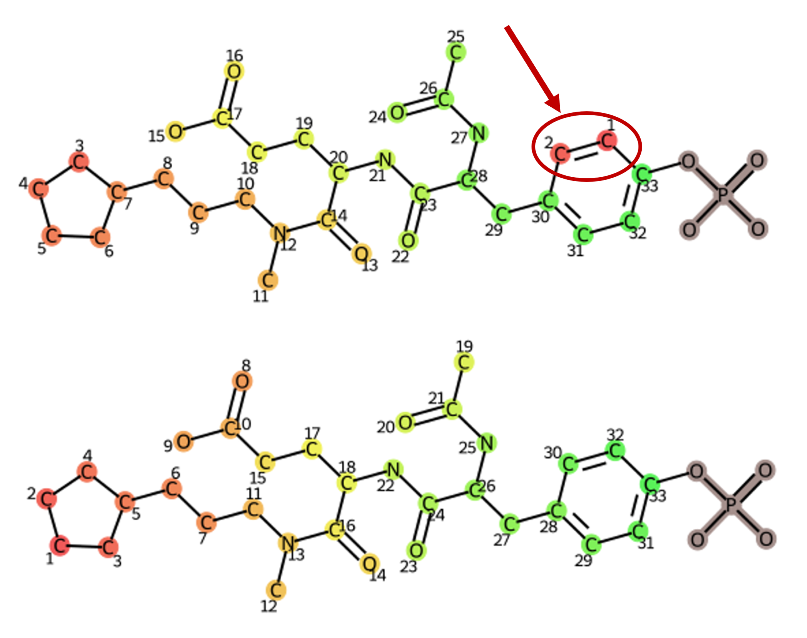
\includegraphics[scale=0.75]{simple_ring_exampledfs2_two_rows}\caption{above: DFS-algorithm; below: BFS-algorithm; CC in dark; the
red arrow indicates the undesired processing of the ring atoms}
\label{fig:simple_ring_exampledfs2}
\end{figure}

\begin{figure}
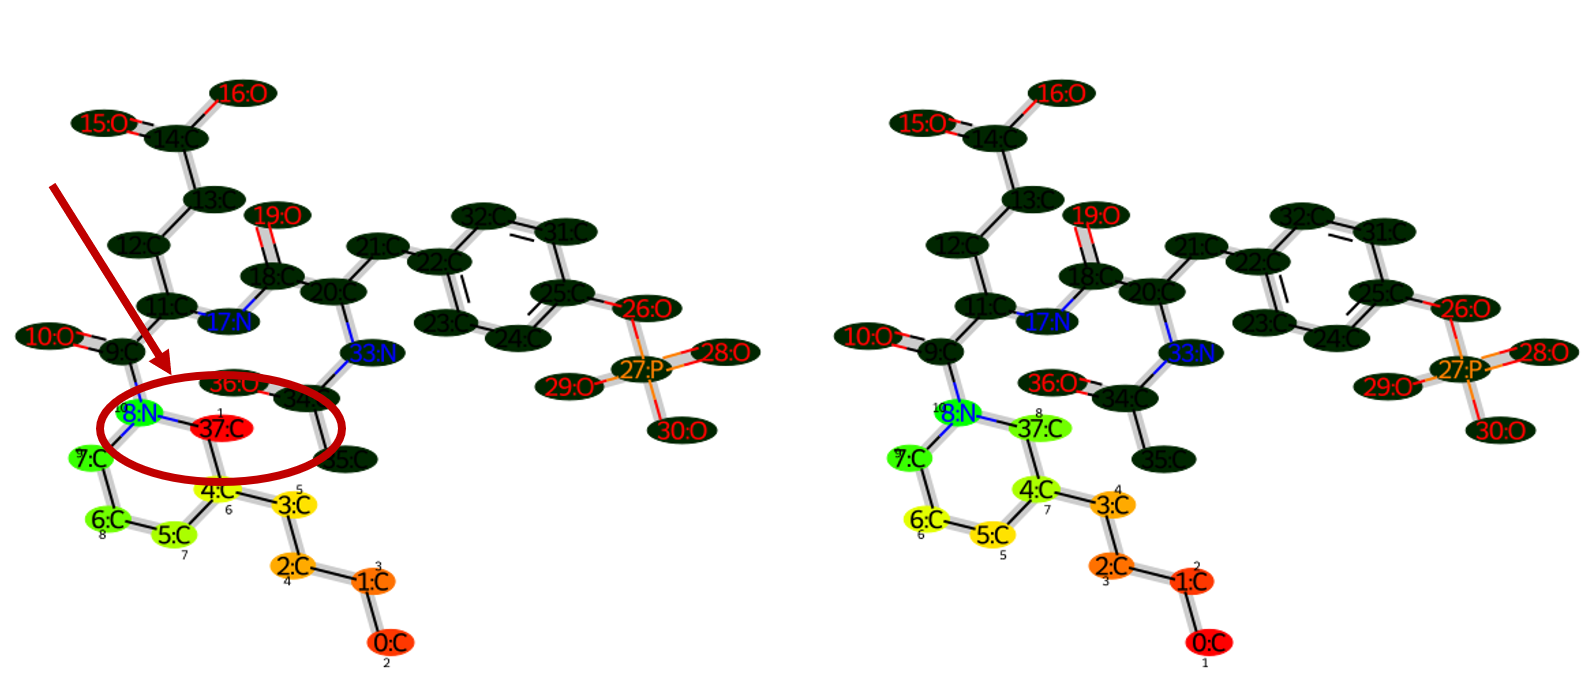
\includegraphics[scale=1.3]{simple_ring_exampledfs3}\caption{left: DFS-algorithm; right: BFS-algorithm; CC in dark; the
red arrow and circle indicates the undesired processing of the ring
atoms}
\label{fig:simple_ring_exampledfs3}
\end{figure}
\begin{figure}

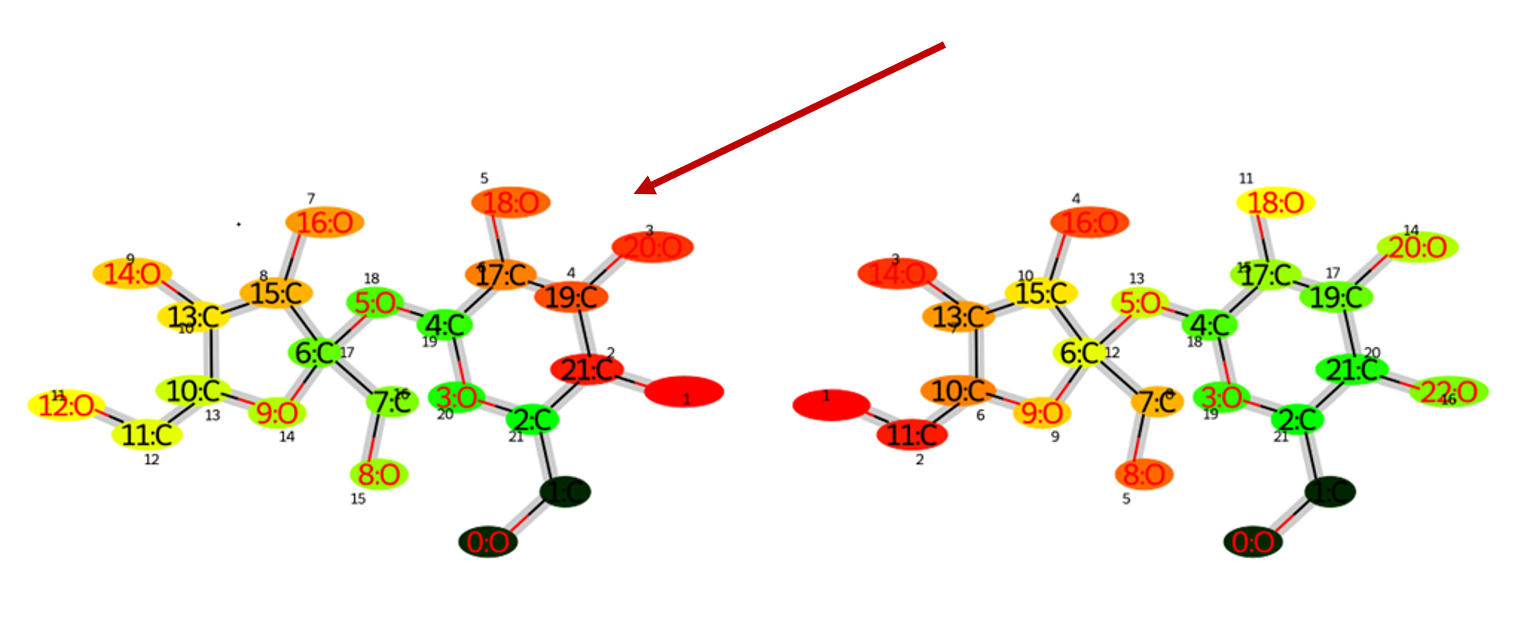
\includegraphics[scale=0.5]{simple_ring_exampledfs4}\caption{left: DFS-algorithm; right: BFS-algorithm; CC in dark; the
red arrow indicates the undesired processing of the ring atoms}
\label{fig:simple_ring_exampledfs4}
\end{figure}

\begin{figure}

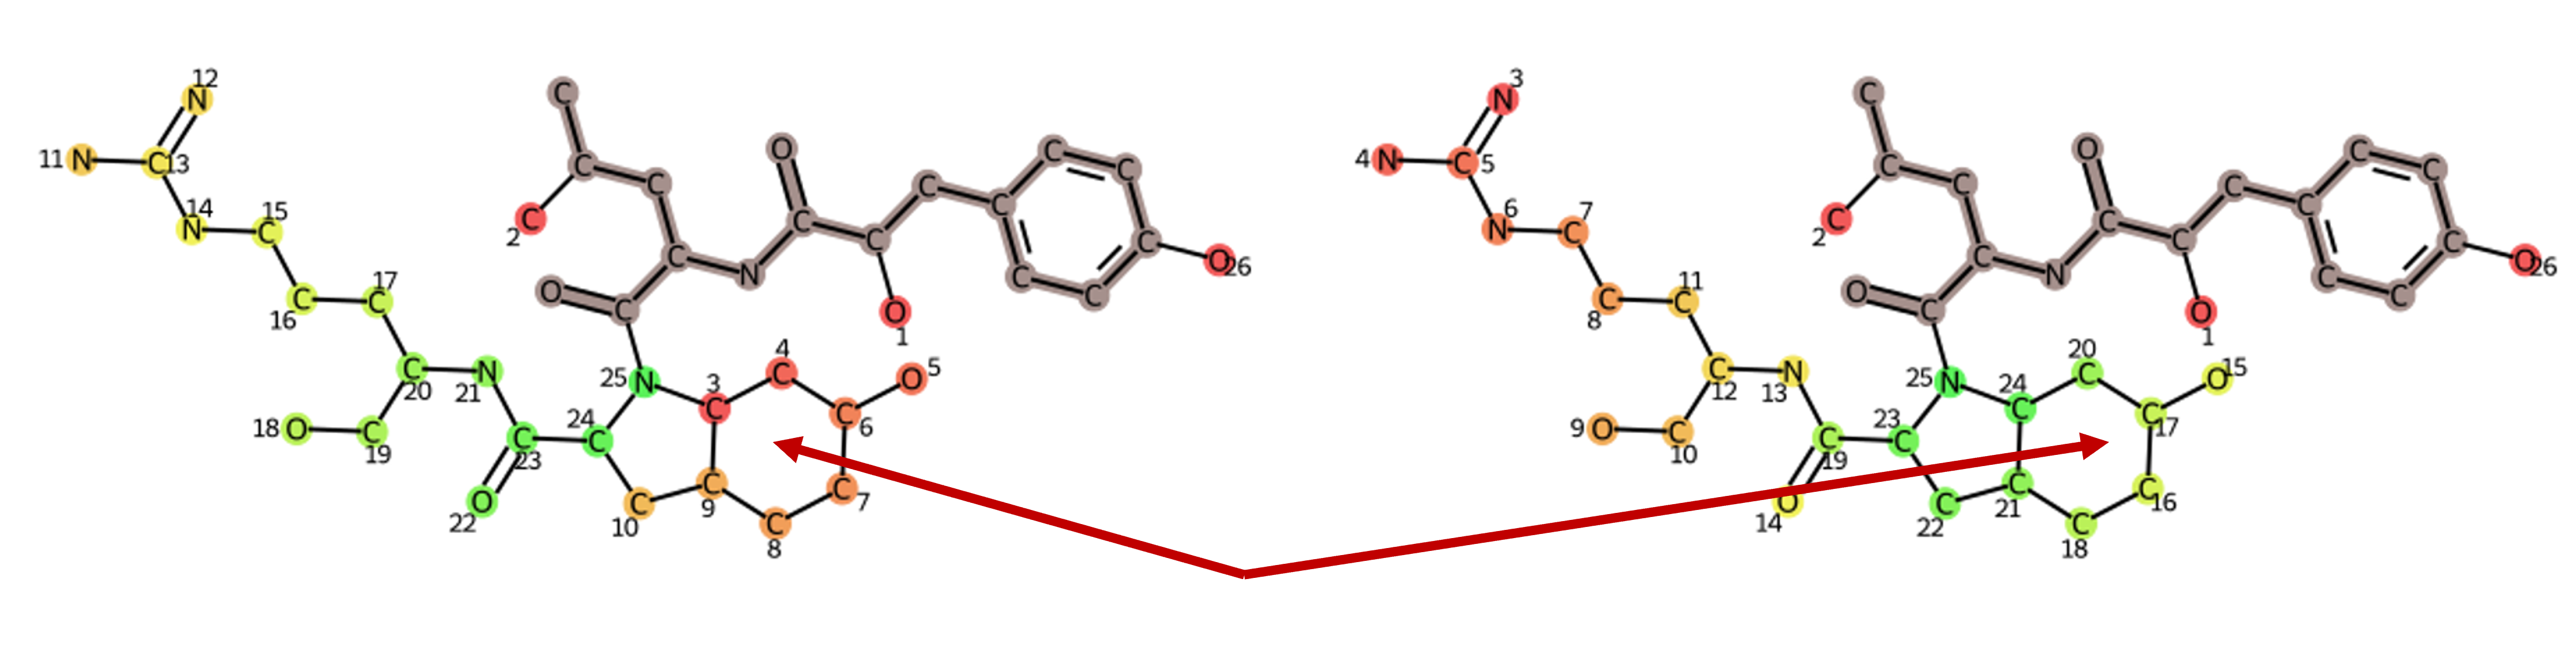
\includegraphics[scale=0.5]{2ring_example}\caption{left: DFS-algorithm; right: BFS-algorithm; CC in dark; the
red arrow indicates the undesired processing of the ring atoms}
\label{fig:2ring_example}
\end{figure}

\begin{figure}

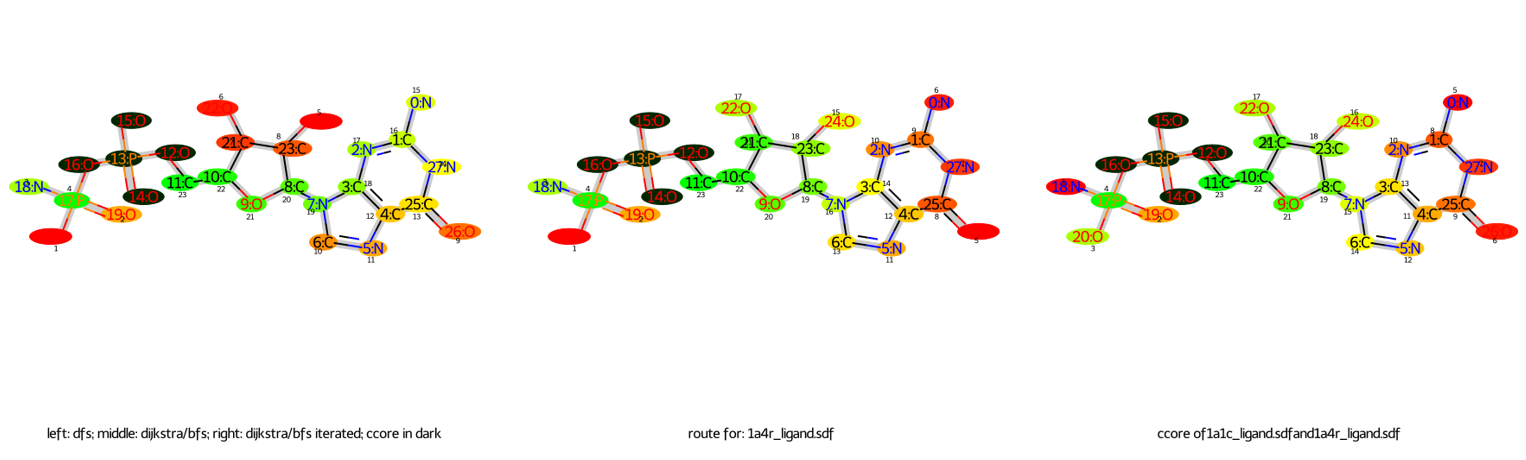
\includegraphics[scale=0.5]{2ring_example2}\caption{left: DFS-algorithm; right: BFS-algorithm; CC in dark; the
red arrow indicates the undesired processing of the ring atoms}
\label{fig:2ring_example2}
\end{figure}
